\documentclass[twoside]{book}

% Packages required by doxygen
\usepackage{fixltx2e}
\usepackage{calc}
\usepackage{doxygen}
\usepackage[export]{adjustbox} % also loads graphicx
\usepackage{graphicx}
\usepackage[utf8]{inputenc}
\usepackage{makeidx}
\usepackage{multicol}
\usepackage{multirow}
\PassOptionsToPackage{warn}{textcomp}
\usepackage{textcomp}
\usepackage[nointegrals]{wasysym}
\usepackage[table]{xcolor}

% Font selection
\usepackage[T1]{fontenc}
\usepackage[scaled=.90]{helvet}
\usepackage{courier}
\usepackage{amssymb}
\usepackage{sectsty}
\renewcommand{\familydefault}{\sfdefault}
\allsectionsfont{%
  \fontseries{bc}\selectfont%
  \color{darkgray}%
}
\renewcommand{\DoxyLabelFont}{%
  \fontseries{bc}\selectfont%
  \color{darkgray}%
}
\newcommand{\+}{\discretionary{\mbox{\scriptsize$\hookleftarrow$}}{}{}}

% Page & text layout
\usepackage{geometry}
\geometry{%
  a4paper,%
  top=2.5cm,%
  bottom=2.5cm,%
  left=2.5cm,%
  right=2.5cm%
}
\tolerance=750
\hfuzz=15pt
\hbadness=750
\setlength{\emergencystretch}{15pt}
\setlength{\parindent}{0cm}
\setlength{\parskip}{0.2cm}
\makeatletter
\renewcommand{\paragraph}{%
  \@startsection{paragraph}{4}{0ex}{-1.0ex}{1.0ex}{%
    \normalfont\normalsize\bfseries\SS@parafont%
  }%
}
\renewcommand{\subparagraph}{%
  \@startsection{subparagraph}{5}{0ex}{-1.0ex}{1.0ex}{%
    \normalfont\normalsize\bfseries\SS@subparafont%
  }%
}
\makeatother

% Headers & footers
\usepackage{fancyhdr}
\pagestyle{fancyplain}
\fancyhead[LE]{\fancyplain{}{\bfseries\thepage}}
\fancyhead[CE]{\fancyplain{}{}}
\fancyhead[RE]{\fancyplain{}{\bfseries\leftmark}}
\fancyhead[LO]{\fancyplain{}{\bfseries\rightmark}}
\fancyhead[CO]{\fancyplain{}{}}
\fancyhead[RO]{\fancyplain{}{\bfseries\thepage}}
\fancyfoot[LE]{\fancyplain{}{}}
\fancyfoot[CE]{\fancyplain{}{}}
\fancyfoot[RE]{\fancyplain{}{\bfseries\scriptsize Generated on Tue Mar 22 2016 10\+:59\+:53 for Open\+C\+L Fluids by Doxygen }}
\fancyfoot[LO]{\fancyplain{}{\bfseries\scriptsize Generated on Tue Mar 22 2016 10\+:59\+:53 for Open\+C\+L Fluids by Doxygen }}
\fancyfoot[CO]{\fancyplain{}{}}
\fancyfoot[RO]{\fancyplain{}{}}
\renewcommand{\footrulewidth}{0.4pt}
\renewcommand{\chaptermark}[1]{%
  \markboth{#1}{}%
}
\renewcommand{\sectionmark}[1]{%
  \markright{\thesection\ #1}%
}

% Indices & bibliography
\usepackage{natbib}
\usepackage[titles]{tocloft}
\setcounter{tocdepth}{3}
\setcounter{secnumdepth}{5}
\makeindex

% Hyperlinks (required, but should be loaded last)
\usepackage{ifpdf}
\ifpdf
  \usepackage[pdftex,pagebackref=true]{hyperref}
\else
  \usepackage[ps2pdf,pagebackref=true]{hyperref}
\fi
\hypersetup{%
  colorlinks=true,%
  linkcolor=blue,%
  citecolor=blue,%
  unicode%
}

% Custom commands
\newcommand{\clearemptydoublepage}{%
  \newpage{\pagestyle{empty}\cleardoublepage}%
}


%===== C O N T E N T S =====

\begin{document}

% Titlepage & ToC
\hypersetup{pageanchor=false,
             bookmarks=true,
             bookmarksnumbered=true,
             pdfencoding=unicode
            }
\pagenumbering{roman}
\begin{titlepage}
\vspace*{7cm}
\begin{center}%
{\Large Open\+C\+L Fluids }\\
\vspace*{1cm}
{\large Generated by Doxygen 1.8.9.1}\\
\vspace*{0.5cm}
{\small Tue Mar 22 2016 10:59:53}\\
\end{center}
\end{titlepage}
\clearemptydoublepage
\tableofcontents
\clearemptydoublepage
\pagenumbering{arabic}
\hypersetup{pageanchor=true}

%--- Begin generated contents ---
\chapter{Hierarchical Index}
\section{Class Hierarchy}
This inheritance list is sorted roughly, but not completely, alphabetically\+:\begin{DoxyCompactList}
\item \contentsline{section}{Device}{\pageref{structDevice}}{}
\item Particle\+System\begin{DoxyCompactList}
\item \contentsline{section}{Solid}{\pageref{classSolid}}{}
\end{DoxyCompactList}
\item \contentsline{section}{Platform}{\pageref{structPlatform}}{}
\item \contentsline{section}{psdata}{\pageref{structpsdata}}{}
\item \contentsline{section}{psdata\+\_\+buf\+List}{\pageref{structpsdata__bufList}}{}
\end{DoxyCompactList}

\chapter{Data Structure Index}
\section{Data Structures}
Here are the data structures with brief descriptions\+:\begin{DoxyCompactList}
\item\contentsline{section}{\hyperlink{structDevice}{Device} }{\pageref{structDevice}}{}
\item\contentsline{section}{\hyperlink{structPlatform}{Platform} }{\pageref{structPlatform}}{}
\item\contentsline{section}{\hyperlink{structpsdata}{psdata} }{\pageref{structpsdata}}{}
\item\contentsline{section}{\hyperlink{structpsdata__bufList}{psdata\+\_\+buf\+List} }{\pageref{structpsdata__bufList}}{}
\item\contentsline{section}{\hyperlink{classSolid}{Solid} }{\pageref{classSolid}}{}
\end{DoxyCompactList}

\chapter{File Index}
\section{File List}
Here is a list of all files with brief descriptions\+:\begin{DoxyCompactList}
\item\contentsline{section}{/home/adam/\+Documents/\+Programming/phd-\/project/opencl-\/implementation/src/\hyperlink{note_8c}{note.\+c} }{\pageref{note_8c}}{}
\item\contentsline{section}{/home/adam/\+Documents/\+Programming/phd-\/project/opencl-\/implementation/src/\hyperlink{note_8h}{note.\+h} }{\pageref{note_8h}}{}
\item\contentsline{section}{/home/adam/\+Documents/\+Programming/phd-\/project/opencl-\/implementation/src/\hyperlink{particle__system_8c}{particle\+\_\+system.\+c} }{\pageref{particle__system_8c}}{}
\item\contentsline{section}{/home/adam/\+Documents/\+Programming/phd-\/project/opencl-\/implementation/src/\hyperlink{particle__system_8h}{particle\+\_\+system.\+h} }{\pageref{particle__system_8h}}{}
\item\contentsline{section}{/home/adam/\+Documents/\+Programming/phd-\/project/opencl-\/implementation/src/\hyperlink{testopencl_8c}{testopencl.\+c} }{\pageref{testopencl_8c}}{}
\item\contentsline{section}{/home/adam/\+Documents/\+Programming/phd-\/project/opencl-\/implementation/src/3rdparty/\hyperlink{whereami_8c}{whereami.\+c} }{\pageref{whereami_8c}}{}
\item\contentsline{section}{/home/adam/\+Documents/\+Programming/phd-\/project/opencl-\/implementation/src/3rdparty/\hyperlink{whereami_8h}{whereami.\+h} }{\pageref{whereami_8h}}{}
\item\contentsline{section}{/home/adam/\+Documents/\+Programming/phd-\/project/opencl-\/implementation/src/mex/\hyperlink{simulation_8c}{simulation.\+c} }{\pageref{simulation_8c}}{}
\item\contentsline{section}{/home/adam/\+Documents/\+Programming/phd-\/project/opencl-\/implementation/src/mex/\hyperlink{simulation_8h}{simulation.\+h} }{\pageref{simulation_8h}}{}
\item\contentsline{section}{/home/adam/\+Documents/\+Programming/phd-\/project/opencl-\/implementation/src/mex/\hyperlink{solid_8h}{solid.\+h} }{\pageref{solid_8h}}{}
\item\contentsline{section}{/home/adam/\+Documents/\+Programming/phd-\/project/opencl-\/implementation/src/mex/\hyperlink{testentry_8c}{testentry.\+c} }{\pageref{testentry_8c}}{}
\item\contentsline{section}{/home/adam/\+Documents/\+Programming/phd-\/project/opencl-\/implementation/src/mex/\hyperlink{testentry2_8c}{testentry2.\+c} }{\pageref{testentry2_8c}}{}
\item\contentsline{section}{/home/adam/\+Documents/\+Programming/phd-\/project/opencl-\/implementation/src/mex/\hyperlink{testentry__wrap_8m}{testentry\+\_\+wrap.\+m} }{\pageref{testentry__wrap_8m}}{}
\item\contentsline{section}{/home/adam/\+Documents/\+Programming/phd-\/project/opencl-\/implementation/src/mex/\hyperlink{testmex_8c}{testmex.\+c} }{\pageref{testmex_8c}}{}
\item\contentsline{section}{/home/adam/\+Documents/\+Programming/phd-\/project/opencl-\/implementation/src/mex/\hyperlink{mex_2testopencl_8c}{testopencl.\+c} }{\pageref{mex_2testopencl_8c}}{}
\item\contentsline{section}{/home/adam/\+Documents/\+Programming/phd-\/project/opencl-\/implementation/src/opencl/\hyperlink{clerror_8c}{clerror.\+c} }{\pageref{clerror_8c}}{}
\item\contentsline{section}{/home/adam/\+Documents/\+Programming/phd-\/project/opencl-\/implementation/src/opencl/\hyperlink{clerror_8h}{clerror.\+h} }{\pageref{clerror_8h}}{}
\item\contentsline{section}{/home/adam/\+Documents/\+Programming/phd-\/project/opencl-\/implementation/src/opencl/\hyperlink{particle__system__host_8c}{particle\+\_\+system\+\_\+host.\+c} }{\pageref{particle__system__host_8c}}{}
\item\contentsline{section}{/home/adam/\+Documents/\+Programming/phd-\/project/opencl-\/implementation/src/opencl/\hyperlink{particle__system__host_8h}{particle\+\_\+system\+\_\+host.\+h} }{\pageref{particle__system__host_8h}}{}
\item\contentsline{section}{/home/adam/\+Documents/\+Programming/phd-\/project/opencl-\/implementation/src/opencl/\hyperlink{platforminfo_8c}{platforminfo.\+c} }{\pageref{platforminfo_8c}}{}
\item\contentsline{section}{/home/adam/\+Documents/\+Programming/phd-\/project/opencl-\/implementation/src/opencl/\hyperlink{platforminfo_8h}{platforminfo.\+h} }{\pageref{platforminfo_8h}}{}
\end{DoxyCompactList}

\chapter{Data Structure Documentation}
\hypertarget{structDevice}{}\section{Device Struct Reference}
\label{structDevice}\index{Device@{Device}}


{\ttfamily \#include $<$platforminfo.\+h$>$}

\subsection*{Data Fields}
\begin{DoxyCompactItemize}
\item 
cl\+\_\+device\+\_\+id \hyperlink{structDevice_ada94aa00c9ab31b8c55bc99061ebfef8}{id}
\item 
char $\ast$ \hyperlink{structDevice_a92d6cdb382fa19b62b961c3ae5288c0b}{name}
\item 
cl\+\_\+device\+\_\+type \hyperlink{structDevice_a4331ce8386201fca48db55cdbe39f94a}{type}
\item 
char $\ast$ \hyperlink{structDevice_a37d2eb2c36cde8a0d35a71ff1b7a9bda}{opencl\+\_\+version}
\item 
char $\ast$ \hyperlink{structDevice_a5b408b26ec962502516f7203a5514145}{driver\+\_\+version}
\item 
char $\ast$ \hyperlink{structDevice_a995dfe3e0fe13c14a3a24dc356ac5db6}{extensions}
\item 
cl\+\_\+bool \hyperlink{structDevice_a4b390bd981afb9c4a6f7f092227129a8}{compiler\+\_\+available}
\item 
cl\+\_\+bool \hyperlink{structDevice_a1edd7c1aaad269999262285f48f5b2a0}{linker\+\_\+available}
\item 
char $\ast$ \hyperlink{structDevice_a8c2887a2df95caba5235491cc8663435}{profile}
\item 
cl\+\_\+uint \hyperlink{structDevice_abb5d5b15973b9b3c64ffe711eefb616c}{max\+\_\+compute\+\_\+units}
\item 
cl\+\_\+uint \hyperlink{structDevice_a6381a5acdd8f3568d1ac6d503ae746d1}{max\+\_\+workgroup\+\_\+size}
\item 
cl\+\_\+uint \hyperlink{structDevice_ad243dd6f35a41309e3856dbb21b7ebf3}{max\+\_\+work\+\_\+item\+\_\+dimensions}
\item 
size\+\_\+t $\ast$ \hyperlink{structDevice_ab86202efb1214bac90b62246ab6dcad2}{max\+\_\+work\+\_\+item\+\_\+sizes}
\item 
cl\+\_\+uint \hyperlink{structDevice_a0fcbcc0f92b61319434da1132cee7045}{pref\+\_\+vector\+\_\+width}
\item 
cl\+\_\+bool \hyperlink{structDevice_a6b660d2db60564f09a267686f3a46ee6}{double\+\_\+supported}
\end{DoxyCompactItemize}


\subsection{Field Documentation}
\hypertarget{structDevice_a4b390bd981afb9c4a6f7f092227129a8}{}\index{Device@{Device}!compiler\+\_\+available@{compiler\+\_\+available}}
\index{compiler\+\_\+available@{compiler\+\_\+available}!Device@{Device}}
\subsubsection[{compiler\+\_\+available}]{\setlength{\rightskip}{0pt plus 5cm}cl\+\_\+bool Device\+::compiler\+\_\+available}\label{structDevice_a4b390bd981afb9c4a6f7f092227129a8}
\hypertarget{structDevice_a6b660d2db60564f09a267686f3a46ee6}{}\index{Device@{Device}!double\+\_\+supported@{double\+\_\+supported}}
\index{double\+\_\+supported@{double\+\_\+supported}!Device@{Device}}
\subsubsection[{double\+\_\+supported}]{\setlength{\rightskip}{0pt plus 5cm}cl\+\_\+bool Device\+::double\+\_\+supported}\label{structDevice_a6b660d2db60564f09a267686f3a46ee6}
\hypertarget{structDevice_a5b408b26ec962502516f7203a5514145}{}\index{Device@{Device}!driver\+\_\+version@{driver\+\_\+version}}
\index{driver\+\_\+version@{driver\+\_\+version}!Device@{Device}}
\subsubsection[{driver\+\_\+version}]{\setlength{\rightskip}{0pt plus 5cm}char$\ast$ Device\+::driver\+\_\+version}\label{structDevice_a5b408b26ec962502516f7203a5514145}
\hypertarget{structDevice_a995dfe3e0fe13c14a3a24dc356ac5db6}{}\index{Device@{Device}!extensions@{extensions}}
\index{extensions@{extensions}!Device@{Device}}
\subsubsection[{extensions}]{\setlength{\rightskip}{0pt plus 5cm}char$\ast$ Device\+::extensions}\label{structDevice_a995dfe3e0fe13c14a3a24dc356ac5db6}
\hypertarget{structDevice_ada94aa00c9ab31b8c55bc99061ebfef8}{}\index{Device@{Device}!id@{id}}
\index{id@{id}!Device@{Device}}
\subsubsection[{id}]{\setlength{\rightskip}{0pt plus 5cm}cl\+\_\+device\+\_\+id Device\+::id}\label{structDevice_ada94aa00c9ab31b8c55bc99061ebfef8}
\hypertarget{structDevice_a1edd7c1aaad269999262285f48f5b2a0}{}\index{Device@{Device}!linker\+\_\+available@{linker\+\_\+available}}
\index{linker\+\_\+available@{linker\+\_\+available}!Device@{Device}}
\subsubsection[{linker\+\_\+available}]{\setlength{\rightskip}{0pt plus 5cm}cl\+\_\+bool Device\+::linker\+\_\+available}\label{structDevice_a1edd7c1aaad269999262285f48f5b2a0}
\hypertarget{structDevice_abb5d5b15973b9b3c64ffe711eefb616c}{}\index{Device@{Device}!max\+\_\+compute\+\_\+units@{max\+\_\+compute\+\_\+units}}
\index{max\+\_\+compute\+\_\+units@{max\+\_\+compute\+\_\+units}!Device@{Device}}
\subsubsection[{max\+\_\+compute\+\_\+units}]{\setlength{\rightskip}{0pt plus 5cm}cl\+\_\+uint Device\+::max\+\_\+compute\+\_\+units}\label{structDevice_abb5d5b15973b9b3c64ffe711eefb616c}
\hypertarget{structDevice_ad243dd6f35a41309e3856dbb21b7ebf3}{}\index{Device@{Device}!max\+\_\+work\+\_\+item\+\_\+dimensions@{max\+\_\+work\+\_\+item\+\_\+dimensions}}
\index{max\+\_\+work\+\_\+item\+\_\+dimensions@{max\+\_\+work\+\_\+item\+\_\+dimensions}!Device@{Device}}
\subsubsection[{max\+\_\+work\+\_\+item\+\_\+dimensions}]{\setlength{\rightskip}{0pt plus 5cm}cl\+\_\+uint Device\+::max\+\_\+work\+\_\+item\+\_\+dimensions}\label{structDevice_ad243dd6f35a41309e3856dbb21b7ebf3}
\hypertarget{structDevice_ab86202efb1214bac90b62246ab6dcad2}{}\index{Device@{Device}!max\+\_\+work\+\_\+item\+\_\+sizes@{max\+\_\+work\+\_\+item\+\_\+sizes}}
\index{max\+\_\+work\+\_\+item\+\_\+sizes@{max\+\_\+work\+\_\+item\+\_\+sizes}!Device@{Device}}
\subsubsection[{max\+\_\+work\+\_\+item\+\_\+sizes}]{\setlength{\rightskip}{0pt plus 5cm}size\+\_\+t$\ast$ Device\+::max\+\_\+work\+\_\+item\+\_\+sizes}\label{structDevice_ab86202efb1214bac90b62246ab6dcad2}
\hypertarget{structDevice_a6381a5acdd8f3568d1ac6d503ae746d1}{}\index{Device@{Device}!max\+\_\+workgroup\+\_\+size@{max\+\_\+workgroup\+\_\+size}}
\index{max\+\_\+workgroup\+\_\+size@{max\+\_\+workgroup\+\_\+size}!Device@{Device}}
\subsubsection[{max\+\_\+workgroup\+\_\+size}]{\setlength{\rightskip}{0pt plus 5cm}cl\+\_\+uint Device\+::max\+\_\+workgroup\+\_\+size}\label{structDevice_a6381a5acdd8f3568d1ac6d503ae746d1}
\hypertarget{structDevice_a92d6cdb382fa19b62b961c3ae5288c0b}{}\index{Device@{Device}!name@{name}}
\index{name@{name}!Device@{Device}}
\subsubsection[{name}]{\setlength{\rightskip}{0pt plus 5cm}char$\ast$ Device\+::name}\label{structDevice_a92d6cdb382fa19b62b961c3ae5288c0b}
\hypertarget{structDevice_a37d2eb2c36cde8a0d35a71ff1b7a9bda}{}\index{Device@{Device}!opencl\+\_\+version@{opencl\+\_\+version}}
\index{opencl\+\_\+version@{opencl\+\_\+version}!Device@{Device}}
\subsubsection[{opencl\+\_\+version}]{\setlength{\rightskip}{0pt plus 5cm}char$\ast$ Device\+::opencl\+\_\+version}\label{structDevice_a37d2eb2c36cde8a0d35a71ff1b7a9bda}
\hypertarget{structDevice_a0fcbcc0f92b61319434da1132cee7045}{}\index{Device@{Device}!pref\+\_\+vector\+\_\+width@{pref\+\_\+vector\+\_\+width}}
\index{pref\+\_\+vector\+\_\+width@{pref\+\_\+vector\+\_\+width}!Device@{Device}}
\subsubsection[{pref\+\_\+vector\+\_\+width}]{\setlength{\rightskip}{0pt plus 5cm}cl\+\_\+uint Device\+::pref\+\_\+vector\+\_\+width}\label{structDevice_a0fcbcc0f92b61319434da1132cee7045}
\hypertarget{structDevice_a8c2887a2df95caba5235491cc8663435}{}\index{Device@{Device}!profile@{profile}}
\index{profile@{profile}!Device@{Device}}
\subsubsection[{profile}]{\setlength{\rightskip}{0pt plus 5cm}char$\ast$ Device\+::profile}\label{structDevice_a8c2887a2df95caba5235491cc8663435}
\hypertarget{structDevice_a4331ce8386201fca48db55cdbe39f94a}{}\index{Device@{Device}!type@{type}}
\index{type@{type}!Device@{Device}}
\subsubsection[{type}]{\setlength{\rightskip}{0pt plus 5cm}cl\+\_\+device\+\_\+type Device\+::type}\label{structDevice_a4331ce8386201fca48db55cdbe39f94a}


The documentation for this struct was generated from the following file\+:\begin{DoxyCompactItemize}
\item 
/home/adam/\+Documents/\+Programming/phd-\/project/opencl-\/implementation/src/opencl/\hyperlink{platforminfo_8h}{platforminfo.\+h}\end{DoxyCompactItemize}

\hypertarget{structPlatform}{}\section{Platform Struct Reference}
\label{structPlatform}\index{Platform@{Platform}}


{\ttfamily \#include $<$platforminfo.\+h$>$}



Collaboration diagram for Platform\+:\nopagebreak
\begin{figure}[H]
\begin{center}
\leavevmode
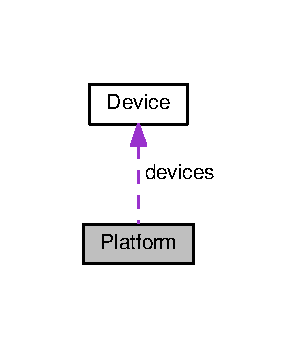
\includegraphics[width=144pt]{structPlatform__coll__graph}
\end{center}
\end{figure}
\subsection*{Data Fields}
\begin{DoxyCompactItemize}
\item 
cl\+\_\+platform\+\_\+id \hyperlink{structPlatform_a4d149e964a154be9bf66784aa1638d87}{id}
\item 
char $\ast$ \hyperlink{structPlatform_a1a3dfb57b0d06ee67684349e1b46631e}{name}
\item 
\hyperlink{structDevice}{Device} const $\ast$ \hyperlink{structPlatform_acdbc822eea50422804f6f8e6de359c0a}{devices}
\item 
unsigned int \hyperlink{structPlatform_a0215aa9a2a4ce8f0ed19ad88a2b6f372}{num\+\_\+devices}
\end{DoxyCompactItemize}


\subsection{Field Documentation}
\hypertarget{structPlatform_acdbc822eea50422804f6f8e6de359c0a}{}\index{Platform@{Platform}!devices@{devices}}
\index{devices@{devices}!Platform@{Platform}}
\subsubsection[{devices}]{\setlength{\rightskip}{0pt plus 5cm}{\bf Device} const$\ast$ Platform\+::devices}\label{structPlatform_acdbc822eea50422804f6f8e6de359c0a}
\hypertarget{structPlatform_a4d149e964a154be9bf66784aa1638d87}{}\index{Platform@{Platform}!id@{id}}
\index{id@{id}!Platform@{Platform}}
\subsubsection[{id}]{\setlength{\rightskip}{0pt plus 5cm}cl\+\_\+platform\+\_\+id Platform\+::id}\label{structPlatform_a4d149e964a154be9bf66784aa1638d87}
\hypertarget{structPlatform_a1a3dfb57b0d06ee67684349e1b46631e}{}\index{Platform@{Platform}!name@{name}}
\index{name@{name}!Platform@{Platform}}
\subsubsection[{name}]{\setlength{\rightskip}{0pt plus 5cm}char$\ast$ Platform\+::name}\label{structPlatform_a1a3dfb57b0d06ee67684349e1b46631e}
\hypertarget{structPlatform_a0215aa9a2a4ce8f0ed19ad88a2b6f372}{}\index{Platform@{Platform}!num\+\_\+devices@{num\+\_\+devices}}
\index{num\+\_\+devices@{num\+\_\+devices}!Platform@{Platform}}
\subsubsection[{num\+\_\+devices}]{\setlength{\rightskip}{0pt plus 5cm}unsigned int Platform\+::num\+\_\+devices}\label{structPlatform_a0215aa9a2a4ce8f0ed19ad88a2b6f372}


The documentation for this struct was generated from the following file\+:\begin{DoxyCompactItemize}
\item 
/home/adam/\+Documents/\+Programming/phd-\/project/opencl-\/implementation/src/opencl/\hyperlink{platforminfo_8h}{platforminfo.\+h}\end{DoxyCompactItemize}

\hypertarget{structpsdata}{}\section{psdata Struct Reference}
\label{structpsdata}\index{psdata@{psdata}}


{\ttfamily \#include $<$particle\+\_\+system.\+h$>$}

\subsection*{Data Fields}
\begin{DoxyCompactItemize}
\item 
unsigned int \hyperlink{structpsdata_a0c5e8cc0fa3042e37da915f97e76dce8}{num\+\_\+fields}
\item 
const char $\ast$ \hyperlink{structpsdata_abfced381a51f5864ab1aaf14f40297ac}{names}
\item 
unsigned int $\ast$ \hyperlink{structpsdata_ad23c8933cb2b7ffd4f44be8d058e73d1}{names\+\_\+offsets}
\item 
unsigned int $\ast$ \hyperlink{structpsdata_a9e5bdb18e75953accfd17efe2c1154ad}{dimensions}
\item 
unsigned int $\ast$ \hyperlink{structpsdata_ad8e436c4ea05c896d8efb2a79ae7bb18}{num\+\_\+dimensions}
\item 
unsigned int $\ast$ \hyperlink{structpsdata_a889d0e2c4ab295832a0480cc6d149619}{dimensions\+\_\+offsets}
\item 
unsigned int $\ast$ \hyperlink{structpsdata_ac507921034797a74a9f5789e70166179}{entry\+\_\+sizes}
\item 
void $\ast$ \hyperlink{structpsdata_aec5fdd50200a11795db62f21f2fedbe7}{data}
\item 
unsigned int $\ast$ \hyperlink{structpsdata_a80714eccad0f11f36babbbaf7360364b}{data\+\_\+sizes}
\item 
unsigned int $\ast$ \hyperlink{structpsdata_a372c86d30fafae1b30546d20f02cf982}{data\+\_\+offsets}
\item 
unsigned int \hyperlink{structpsdata_a4b71cba344ccd849f7ae01779b9338a7}{num\+\_\+host\+\_\+fields}
\item 
char $\ast$$\ast$ \hyperlink{structpsdata_a8209dbc814fce6a98341f682d92581a9}{host\+\_\+names}
\item 
void $\ast$$\ast$ \hyperlink{structpsdata_aa7f64559ff6379b1cbc744634687dc26}{host\+\_\+data}
\item 
unsigned int $\ast$ \hyperlink{structpsdata_ae9e934a711b985fee410829e02acedc9}{host\+\_\+data\+\_\+size}
\end{DoxyCompactItemize}


\subsection{Field Documentation}
\hypertarget{structpsdata_aec5fdd50200a11795db62f21f2fedbe7}{}\index{psdata@{psdata}!data@{data}}
\index{data@{data}!psdata@{psdata}}
\subsubsection[{data}]{\setlength{\rightskip}{0pt plus 5cm}void$\ast$ psdata\+::data}\label{structpsdata_aec5fdd50200a11795db62f21f2fedbe7}
\hypertarget{structpsdata_a372c86d30fafae1b30546d20f02cf982}{}\index{psdata@{psdata}!data\+\_\+offsets@{data\+\_\+offsets}}
\index{data\+\_\+offsets@{data\+\_\+offsets}!psdata@{psdata}}
\subsubsection[{data\+\_\+offsets}]{\setlength{\rightskip}{0pt plus 5cm}unsigned int$\ast$ psdata\+::data\+\_\+offsets}\label{structpsdata_a372c86d30fafae1b30546d20f02cf982}
\hypertarget{structpsdata_a80714eccad0f11f36babbbaf7360364b}{}\index{psdata@{psdata}!data\+\_\+sizes@{data\+\_\+sizes}}
\index{data\+\_\+sizes@{data\+\_\+sizes}!psdata@{psdata}}
\subsubsection[{data\+\_\+sizes}]{\setlength{\rightskip}{0pt plus 5cm}unsigned int$\ast$ psdata\+::data\+\_\+sizes}\label{structpsdata_a80714eccad0f11f36babbbaf7360364b}
\hypertarget{structpsdata_a9e5bdb18e75953accfd17efe2c1154ad}{}\index{psdata@{psdata}!dimensions@{dimensions}}
\index{dimensions@{dimensions}!psdata@{psdata}}
\subsubsection[{dimensions}]{\setlength{\rightskip}{0pt plus 5cm}unsigned int$\ast$ psdata\+::dimensions}\label{structpsdata_a9e5bdb18e75953accfd17efe2c1154ad}
\hypertarget{structpsdata_a889d0e2c4ab295832a0480cc6d149619}{}\index{psdata@{psdata}!dimensions\+\_\+offsets@{dimensions\+\_\+offsets}}
\index{dimensions\+\_\+offsets@{dimensions\+\_\+offsets}!psdata@{psdata}}
\subsubsection[{dimensions\+\_\+offsets}]{\setlength{\rightskip}{0pt plus 5cm}unsigned int$\ast$ psdata\+::dimensions\+\_\+offsets}\label{structpsdata_a889d0e2c4ab295832a0480cc6d149619}
\hypertarget{structpsdata_ac507921034797a74a9f5789e70166179}{}\index{psdata@{psdata}!entry\+\_\+sizes@{entry\+\_\+sizes}}
\index{entry\+\_\+sizes@{entry\+\_\+sizes}!psdata@{psdata}}
\subsubsection[{entry\+\_\+sizes}]{\setlength{\rightskip}{0pt plus 5cm}unsigned int$\ast$ psdata\+::entry\+\_\+sizes}\label{structpsdata_ac507921034797a74a9f5789e70166179}
\hypertarget{structpsdata_aa7f64559ff6379b1cbc744634687dc26}{}\index{psdata@{psdata}!host\+\_\+data@{host\+\_\+data}}
\index{host\+\_\+data@{host\+\_\+data}!psdata@{psdata}}
\subsubsection[{host\+\_\+data}]{\setlength{\rightskip}{0pt plus 5cm}void$\ast$$\ast$ psdata\+::host\+\_\+data}\label{structpsdata_aa7f64559ff6379b1cbc744634687dc26}
\hypertarget{structpsdata_ae9e934a711b985fee410829e02acedc9}{}\index{psdata@{psdata}!host\+\_\+data\+\_\+size@{host\+\_\+data\+\_\+size}}
\index{host\+\_\+data\+\_\+size@{host\+\_\+data\+\_\+size}!psdata@{psdata}}
\subsubsection[{host\+\_\+data\+\_\+size}]{\setlength{\rightskip}{0pt plus 5cm}unsigned int$\ast$ psdata\+::host\+\_\+data\+\_\+size}\label{structpsdata_ae9e934a711b985fee410829e02acedc9}
\hypertarget{structpsdata_a8209dbc814fce6a98341f682d92581a9}{}\index{psdata@{psdata}!host\+\_\+names@{host\+\_\+names}}
\index{host\+\_\+names@{host\+\_\+names}!psdata@{psdata}}
\subsubsection[{host\+\_\+names}]{\setlength{\rightskip}{0pt plus 5cm}char$\ast$$\ast$ psdata\+::host\+\_\+names}\label{structpsdata_a8209dbc814fce6a98341f682d92581a9}
\hypertarget{structpsdata_abfced381a51f5864ab1aaf14f40297ac}{}\index{psdata@{psdata}!names@{names}}
\index{names@{names}!psdata@{psdata}}
\subsubsection[{names}]{\setlength{\rightskip}{0pt plus 5cm}const char$\ast$ psdata\+::names}\label{structpsdata_abfced381a51f5864ab1aaf14f40297ac}
\hypertarget{structpsdata_ad23c8933cb2b7ffd4f44be8d058e73d1}{}\index{psdata@{psdata}!names\+\_\+offsets@{names\+\_\+offsets}}
\index{names\+\_\+offsets@{names\+\_\+offsets}!psdata@{psdata}}
\subsubsection[{names\+\_\+offsets}]{\setlength{\rightskip}{0pt plus 5cm}unsigned int$\ast$ psdata\+::names\+\_\+offsets}\label{structpsdata_ad23c8933cb2b7ffd4f44be8d058e73d1}
\hypertarget{structpsdata_ad8e436c4ea05c896d8efb2a79ae7bb18}{}\index{psdata@{psdata}!num\+\_\+dimensions@{num\+\_\+dimensions}}
\index{num\+\_\+dimensions@{num\+\_\+dimensions}!psdata@{psdata}}
\subsubsection[{num\+\_\+dimensions}]{\setlength{\rightskip}{0pt plus 5cm}unsigned int$\ast$ psdata\+::num\+\_\+dimensions}\label{structpsdata_ad8e436c4ea05c896d8efb2a79ae7bb18}
\hypertarget{structpsdata_a0c5e8cc0fa3042e37da915f97e76dce8}{}\index{psdata@{psdata}!num\+\_\+fields@{num\+\_\+fields}}
\index{num\+\_\+fields@{num\+\_\+fields}!psdata@{psdata}}
\subsubsection[{num\+\_\+fields}]{\setlength{\rightskip}{0pt plus 5cm}unsigned int psdata\+::num\+\_\+fields}\label{structpsdata_a0c5e8cc0fa3042e37da915f97e76dce8}
The numerical data is all stored in a contiguous array at data, to facilitate uploading to the G\+P\+U.

When data needs to be used by M\+A\+T\+L\+A\+B, sync\+\_\+to\+\_\+mex should be used to copy the flat stored data to the M\+E\+X managed arrays in host\+\_\+data. These are kept host-\/side throughout as I don\textquotesingle{}t know anything about their internal structure. \hypertarget{structpsdata_a4b71cba344ccd849f7ae01779b9338a7}{}\index{psdata@{psdata}!num\+\_\+host\+\_\+fields@{num\+\_\+host\+\_\+fields}}
\index{num\+\_\+host\+\_\+fields@{num\+\_\+host\+\_\+fields}!psdata@{psdata}}
\subsubsection[{num\+\_\+host\+\_\+fields}]{\setlength{\rightskip}{0pt plus 5cm}unsigned int psdata\+::num\+\_\+host\+\_\+fields}\label{structpsdata_a4b71cba344ccd849f7ae01779b9338a7}


The documentation for this struct was generated from the following file\+:\begin{DoxyCompactItemize}
\item 
/home/adam/\+Documents/\+Programming/phd-\/project/opencl-\/implementation/src/\hyperlink{particle__system_8h}{particle\+\_\+system.\+h}\end{DoxyCompactItemize}

\hypertarget{structpsdata__bufList}{}\section{psdata\+\_\+buf\+List Struct Reference}
\label{structpsdata__bufList}\index{psdata\+\_\+buf\+List@{psdata\+\_\+buf\+List}}


{\ttfamily \#include $<$particle\+\_\+system\+\_\+host.\+h$>$}

\subsection*{Data Fields}
\begin{DoxyCompactItemize}
\item 
unsigned int \hyperlink{structpsdata__bufList_a8150194819034d266db259d3469e3093}{num\+\_\+fields}
\item 
cl\+\_\+mem \hyperlink{structpsdata__bufList_a692e26c884416e7b932f2785eb0a9f97}{names}
\item 
cl\+\_\+mem \hyperlink{structpsdata__bufList_a959534753c9b5429408fdb1c99f4479c}{names\+\_\+offsets}
\item 
cl\+\_\+mem \hyperlink{structpsdata__bufList_affc6b6790b65adc5ffd41ffe654477e7}{dimensions}
\item 
cl\+\_\+mem \hyperlink{structpsdata__bufList_ab88f6bd66f625383d9781707d266cd66}{num\+\_\+dimensions}
\item 
cl\+\_\+mem \hyperlink{structpsdata__bufList_af2352e065d080b867a1aea92db81dca8}{dimensions\+\_\+offsets}
\item 
cl\+\_\+mem \hyperlink{structpsdata__bufList_a887652ee87b5f358abf6ad65f37b4800}{entry\+\_\+sizes}
\item 
cl\+\_\+mem \hyperlink{structpsdata__bufList_ab2931ac0677c25cc9885e7dc9964b088}{data}
\item 
cl\+\_\+mem \hyperlink{structpsdata__bufList_af4f580f6a6cdfe8f4894d596c1665578}{data\+\_\+sizes}
\item 
cl\+\_\+mem \hyperlink{structpsdata__bufList_a349d575ccdb00eddbab74a6f0590a90d}{data\+\_\+offsets}
\end{DoxyCompactItemize}


\subsection{Field Documentation}
\hypertarget{structpsdata__bufList_ab2931ac0677c25cc9885e7dc9964b088}{}\index{psdata\+\_\+buf\+List@{psdata\+\_\+buf\+List}!data@{data}}
\index{data@{data}!psdata\+\_\+buf\+List@{psdata\+\_\+buf\+List}}
\subsubsection[{data}]{\setlength{\rightskip}{0pt plus 5cm}cl\+\_\+mem psdata\+\_\+buf\+List\+::data}\label{structpsdata__bufList_ab2931ac0677c25cc9885e7dc9964b088}
\hypertarget{structpsdata__bufList_a349d575ccdb00eddbab74a6f0590a90d}{}\index{psdata\+\_\+buf\+List@{psdata\+\_\+buf\+List}!data\+\_\+offsets@{data\+\_\+offsets}}
\index{data\+\_\+offsets@{data\+\_\+offsets}!psdata\+\_\+buf\+List@{psdata\+\_\+buf\+List}}
\subsubsection[{data\+\_\+offsets}]{\setlength{\rightskip}{0pt plus 5cm}cl\+\_\+mem psdata\+\_\+buf\+List\+::data\+\_\+offsets}\label{structpsdata__bufList_a349d575ccdb00eddbab74a6f0590a90d}
\hypertarget{structpsdata__bufList_af4f580f6a6cdfe8f4894d596c1665578}{}\index{psdata\+\_\+buf\+List@{psdata\+\_\+buf\+List}!data\+\_\+sizes@{data\+\_\+sizes}}
\index{data\+\_\+sizes@{data\+\_\+sizes}!psdata\+\_\+buf\+List@{psdata\+\_\+buf\+List}}
\subsubsection[{data\+\_\+sizes}]{\setlength{\rightskip}{0pt plus 5cm}cl\+\_\+mem psdata\+\_\+buf\+List\+::data\+\_\+sizes}\label{structpsdata__bufList_af4f580f6a6cdfe8f4894d596c1665578}
\hypertarget{structpsdata__bufList_affc6b6790b65adc5ffd41ffe654477e7}{}\index{psdata\+\_\+buf\+List@{psdata\+\_\+buf\+List}!dimensions@{dimensions}}
\index{dimensions@{dimensions}!psdata\+\_\+buf\+List@{psdata\+\_\+buf\+List}}
\subsubsection[{dimensions}]{\setlength{\rightskip}{0pt plus 5cm}cl\+\_\+mem psdata\+\_\+buf\+List\+::dimensions}\label{structpsdata__bufList_affc6b6790b65adc5ffd41ffe654477e7}
\hypertarget{structpsdata__bufList_af2352e065d080b867a1aea92db81dca8}{}\index{psdata\+\_\+buf\+List@{psdata\+\_\+buf\+List}!dimensions\+\_\+offsets@{dimensions\+\_\+offsets}}
\index{dimensions\+\_\+offsets@{dimensions\+\_\+offsets}!psdata\+\_\+buf\+List@{psdata\+\_\+buf\+List}}
\subsubsection[{dimensions\+\_\+offsets}]{\setlength{\rightskip}{0pt plus 5cm}cl\+\_\+mem psdata\+\_\+buf\+List\+::dimensions\+\_\+offsets}\label{structpsdata__bufList_af2352e065d080b867a1aea92db81dca8}
\hypertarget{structpsdata__bufList_a887652ee87b5f358abf6ad65f37b4800}{}\index{psdata\+\_\+buf\+List@{psdata\+\_\+buf\+List}!entry\+\_\+sizes@{entry\+\_\+sizes}}
\index{entry\+\_\+sizes@{entry\+\_\+sizes}!psdata\+\_\+buf\+List@{psdata\+\_\+buf\+List}}
\subsubsection[{entry\+\_\+sizes}]{\setlength{\rightskip}{0pt plus 5cm}cl\+\_\+mem psdata\+\_\+buf\+List\+::entry\+\_\+sizes}\label{structpsdata__bufList_a887652ee87b5f358abf6ad65f37b4800}
\hypertarget{structpsdata__bufList_a692e26c884416e7b932f2785eb0a9f97}{}\index{psdata\+\_\+buf\+List@{psdata\+\_\+buf\+List}!names@{names}}
\index{names@{names}!psdata\+\_\+buf\+List@{psdata\+\_\+buf\+List}}
\subsubsection[{names}]{\setlength{\rightskip}{0pt plus 5cm}cl\+\_\+mem psdata\+\_\+buf\+List\+::names}\label{structpsdata__bufList_a692e26c884416e7b932f2785eb0a9f97}
\hypertarget{structpsdata__bufList_a959534753c9b5429408fdb1c99f4479c}{}\index{psdata\+\_\+buf\+List@{psdata\+\_\+buf\+List}!names\+\_\+offsets@{names\+\_\+offsets}}
\index{names\+\_\+offsets@{names\+\_\+offsets}!psdata\+\_\+buf\+List@{psdata\+\_\+buf\+List}}
\subsubsection[{names\+\_\+offsets}]{\setlength{\rightskip}{0pt plus 5cm}cl\+\_\+mem psdata\+\_\+buf\+List\+::names\+\_\+offsets}\label{structpsdata__bufList_a959534753c9b5429408fdb1c99f4479c}
\hypertarget{structpsdata__bufList_ab88f6bd66f625383d9781707d266cd66}{}\index{psdata\+\_\+buf\+List@{psdata\+\_\+buf\+List}!num\+\_\+dimensions@{num\+\_\+dimensions}}
\index{num\+\_\+dimensions@{num\+\_\+dimensions}!psdata\+\_\+buf\+List@{psdata\+\_\+buf\+List}}
\subsubsection[{num\+\_\+dimensions}]{\setlength{\rightskip}{0pt plus 5cm}cl\+\_\+mem psdata\+\_\+buf\+List\+::num\+\_\+dimensions}\label{structpsdata__bufList_ab88f6bd66f625383d9781707d266cd66}
\hypertarget{structpsdata__bufList_a8150194819034d266db259d3469e3093}{}\index{psdata\+\_\+buf\+List@{psdata\+\_\+buf\+List}!num\+\_\+fields@{num\+\_\+fields}}
\index{num\+\_\+fields@{num\+\_\+fields}!psdata\+\_\+buf\+List@{psdata\+\_\+buf\+List}}
\subsubsection[{num\+\_\+fields}]{\setlength{\rightskip}{0pt plus 5cm}unsigned int psdata\+\_\+buf\+List\+::num\+\_\+fields}\label{structpsdata__bufList_a8150194819034d266db259d3469e3093}


The documentation for this struct was generated from the following file\+:\begin{DoxyCompactItemize}
\item 
/home/adam/\+Documents/\+Programming/phd-\/project/opencl-\/implementation/src/opencl/\hyperlink{particle__system__host_8h}{particle\+\_\+system\+\_\+host.\+h}\end{DoxyCompactItemize}

\hypertarget{classSolid}{}\section{Solid Class Reference}
\label{classSolid}\index{Solid@{Solid}}


{\ttfamily \#include $<$solid.\+h$>$}



Inheritance diagram for Solid\+:\nopagebreak
\begin{figure}[H]
\begin{center}
\leavevmode
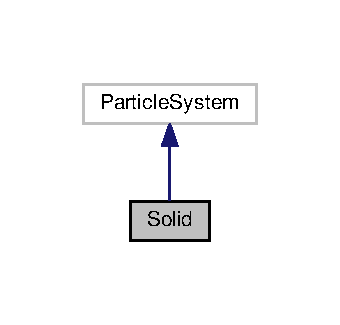
\includegraphics[width=163pt]{classSolid__inherit__graph}
\end{center}
\end{figure}


Collaboration diagram for Solid\+:\nopagebreak
\begin{figure}[H]
\begin{center}
\leavevmode
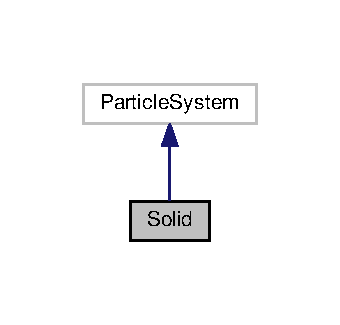
\includegraphics[width=163pt]{classSolid__coll__graph}
\end{center}
\end{figure}


The documentation for this class was generated from the following file\+:\begin{DoxyCompactItemize}
\item 
/home/adam/\+Documents/\+Programming/phd-\/project/opencl-\/implementation/src/mex/\hyperlink{solid_8h}{solid.\+h}\end{DoxyCompactItemize}

\chapter{File Documentation}
\hypertarget{whereami_8c}{}\section{/home/adam/\+Documents/\+Programming/phd-\/project/opencl-\/implementation/src/3rdparty/whereami.c File Reference}
\label{whereami_8c}\index{/home/adam/\+Documents/\+Programming/phd-\/project/opencl-\/implementation/src/3rdparty/whereami.\+c@{/home/adam/\+Documents/\+Programming/phd-\/project/opencl-\/implementation/src/3rdparty/whereami.\+c}}
{\ttfamily \#include \char`\"{}whereami.\+h\char`\"{}}\\*
{\ttfamily \#include $<$stdlib.\+h$>$}\\*
Include dependency graph for whereami.\+c\+:
\nopagebreak
\begin{figure}[H]
\begin{center}
\leavevmode
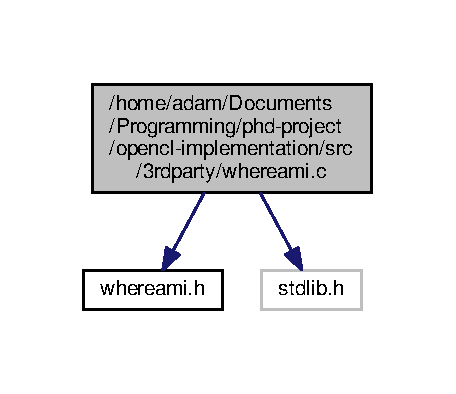
\includegraphics[width=219pt]{whereami_8c__incl}
\end{center}
\end{figure}
\subsection*{Macros}
\begin{DoxyCompactItemize}
\item 
\#define \hyperlink{whereami_8c_a39b37162eaf1ae5b907b22c1d0eaeb14}{W\+A\+I\+\_\+\+M\+A\+L\+L\+O\+C}(size)~malloc(size)
\item 
\#define \hyperlink{whereami_8c_a98f334c08ee3125a5b327006826b0faa}{W\+A\+I\+\_\+\+F\+R\+E\+E}(p)~free(p)
\item 
\#define \hyperlink{whereami_8c_af54ad0f7a94f67e1ba5f927387794bb4}{W\+A\+I\+\_\+\+R\+E\+A\+L\+L\+O\+C}(p,  size)~realloc(p, size)
\end{DoxyCompactItemize}


\subsection{Macro Definition Documentation}
\hypertarget{whereami_8c_a98f334c08ee3125a5b327006826b0faa}{}\index{whereami.\+c@{whereami.\+c}!W\+A\+I\+\_\+\+F\+R\+E\+E@{W\+A\+I\+\_\+\+F\+R\+E\+E}}
\index{W\+A\+I\+\_\+\+F\+R\+E\+E@{W\+A\+I\+\_\+\+F\+R\+E\+E}!whereami.\+c@{whereami.\+c}}
\subsubsection[{W\+A\+I\+\_\+\+F\+R\+E\+E}]{\setlength{\rightskip}{0pt plus 5cm}\#define W\+A\+I\+\_\+\+F\+R\+E\+E(
\begin{DoxyParamCaption}
\item[{}]{p}
\end{DoxyParamCaption}
)~free(p)}\label{whereami_8c_a98f334c08ee3125a5b327006826b0faa}
\hypertarget{whereami_8c_a39b37162eaf1ae5b907b22c1d0eaeb14}{}\index{whereami.\+c@{whereami.\+c}!W\+A\+I\+\_\+\+M\+A\+L\+L\+O\+C@{W\+A\+I\+\_\+\+M\+A\+L\+L\+O\+C}}
\index{W\+A\+I\+\_\+\+M\+A\+L\+L\+O\+C@{W\+A\+I\+\_\+\+M\+A\+L\+L\+O\+C}!whereami.\+c@{whereami.\+c}}
\subsubsection[{W\+A\+I\+\_\+\+M\+A\+L\+L\+O\+C}]{\setlength{\rightskip}{0pt plus 5cm}\#define W\+A\+I\+\_\+\+M\+A\+L\+L\+O\+C(
\begin{DoxyParamCaption}
\item[{}]{size}
\end{DoxyParamCaption}
)~malloc(size)}\label{whereami_8c_a39b37162eaf1ae5b907b22c1d0eaeb14}
\hypertarget{whereami_8c_af54ad0f7a94f67e1ba5f927387794bb4}{}\index{whereami.\+c@{whereami.\+c}!W\+A\+I\+\_\+\+R\+E\+A\+L\+L\+O\+C@{W\+A\+I\+\_\+\+R\+E\+A\+L\+L\+O\+C}}
\index{W\+A\+I\+\_\+\+R\+E\+A\+L\+L\+O\+C@{W\+A\+I\+\_\+\+R\+E\+A\+L\+L\+O\+C}!whereami.\+c@{whereami.\+c}}
\subsubsection[{W\+A\+I\+\_\+\+R\+E\+A\+L\+L\+O\+C}]{\setlength{\rightskip}{0pt plus 5cm}\#define W\+A\+I\+\_\+\+R\+E\+A\+L\+L\+O\+C(
\begin{DoxyParamCaption}
\item[{}]{p, }
\item[{}]{size}
\end{DoxyParamCaption}
)~realloc(p, size)}\label{whereami_8c_af54ad0f7a94f67e1ba5f927387794bb4}

\hypertarget{whereami_8h}{}\section{/home/adam/\+Documents/\+Programming/phd-\/project/opencl-\/implementation/src/3rdparty/whereami.h File Reference}
\label{whereami_8h}\index{/home/adam/\+Documents/\+Programming/phd-\/project/opencl-\/implementation/src/3rdparty/whereami.\+h@{/home/adam/\+Documents/\+Programming/phd-\/project/opencl-\/implementation/src/3rdparty/whereami.\+h}}
This graph shows which files directly or indirectly include this file\+:
\nopagebreak
\begin{figure}[H]
\begin{center}
\leavevmode
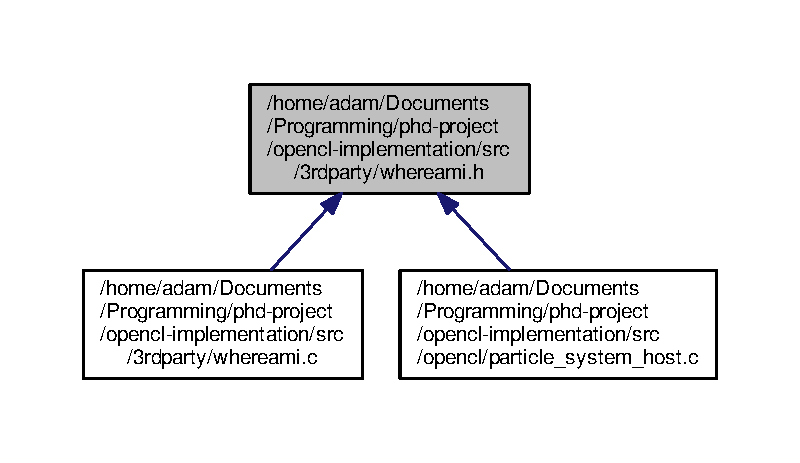
\includegraphics[width=350pt]{whereami_8h__dep__incl}
\end{center}
\end{figure}
\subsection*{Macros}
\begin{DoxyCompactItemize}
\item 
\#define \hyperlink{whereami_8h_af4a5433582844c6d1f4e5f48e911fe02}{W\+A\+I\+\_\+\+F\+U\+N\+C\+S\+P\+E\+C}
\item 
\#define \hyperlink{whereami_8h_aca46f8ead8100022a86fa699ccffab93}{W\+A\+I\+\_\+\+P\+R\+E\+F\+I\+X}(function)~wai\+\_\+\#\#function
\end{DoxyCompactItemize}
\subsection*{Functions}
\begin{DoxyCompactItemize}
\item 
\hyperlink{whereami_8h_af4a5433582844c6d1f4e5f48e911fe02}{W\+A\+I\+\_\+\+F\+U\+N\+C\+S\+P\+E\+C} int \hyperlink{whereami_8h_aca46f8ead8100022a86fa699ccffab93}{W\+A\+I\+\_\+\+P\+R\+E\+F\+I\+X}() \hyperlink{whereami_8h_a1d7105bf3f056c5cf45b8d4bab266216}{get\+Executable\+Path} (char $\ast$out, int capacity, int $\ast$dirname\+\_\+length)
\item 
\hyperlink{whereami_8h_af4a5433582844c6d1f4e5f48e911fe02}{W\+A\+I\+\_\+\+F\+U\+N\+C\+S\+P\+E\+C} int \hyperlink{whereami_8h_aca46f8ead8100022a86fa699ccffab93}{W\+A\+I\+\_\+\+P\+R\+E\+F\+I\+X}() \hyperlink{whereami_8h_a3e646ad33f266a102996d0e9c5155eca}{get\+Module\+Path} (char $\ast$out, int capacity, int $\ast$dirname\+\_\+length)
\end{DoxyCompactItemize}


\subsection{Macro Definition Documentation}
\hypertarget{whereami_8h_af4a5433582844c6d1f4e5f48e911fe02}{}\index{whereami.\+h@{whereami.\+h}!W\+A\+I\+\_\+\+F\+U\+N\+C\+S\+P\+E\+C@{W\+A\+I\+\_\+\+F\+U\+N\+C\+S\+P\+E\+C}}
\index{W\+A\+I\+\_\+\+F\+U\+N\+C\+S\+P\+E\+C@{W\+A\+I\+\_\+\+F\+U\+N\+C\+S\+P\+E\+C}!whereami.\+h@{whereami.\+h}}
\subsubsection[{W\+A\+I\+\_\+\+F\+U\+N\+C\+S\+P\+E\+C}]{\setlength{\rightskip}{0pt plus 5cm}\#define W\+A\+I\+\_\+\+F\+U\+N\+C\+S\+P\+E\+C}\label{whereami_8h_af4a5433582844c6d1f4e5f48e911fe02}
\hypertarget{whereami_8h_aca46f8ead8100022a86fa699ccffab93}{}\index{whereami.\+h@{whereami.\+h}!W\+A\+I\+\_\+\+P\+R\+E\+F\+I\+X@{W\+A\+I\+\_\+\+P\+R\+E\+F\+I\+X}}
\index{W\+A\+I\+\_\+\+P\+R\+E\+F\+I\+X@{W\+A\+I\+\_\+\+P\+R\+E\+F\+I\+X}!whereami.\+h@{whereami.\+h}}
\subsubsection[{W\+A\+I\+\_\+\+P\+R\+E\+F\+I\+X}]{\setlength{\rightskip}{0pt plus 5cm}\#define W\+A\+I\+\_\+\+P\+R\+E\+F\+I\+X(
\begin{DoxyParamCaption}
\item[{}]{function}
\end{DoxyParamCaption}
)~wai\+\_\+\#\#function}\label{whereami_8h_aca46f8ead8100022a86fa699ccffab93}


\subsection{Function Documentation}
\hypertarget{whereami_8h_a1d7105bf3f056c5cf45b8d4bab266216}{}\index{whereami.\+h@{whereami.\+h}!get\+Executable\+Path@{get\+Executable\+Path}}
\index{get\+Executable\+Path@{get\+Executable\+Path}!whereami.\+h@{whereami.\+h}}
\subsubsection[{get\+Executable\+Path}]{\setlength{\rightskip}{0pt plus 5cm}{\bf W\+A\+I\+\_\+\+F\+U\+N\+C\+S\+P\+E\+C} int {\bf W\+A\+I\+\_\+\+P\+R\+E\+F\+I\+X}() get\+Executable\+Path (
\begin{DoxyParamCaption}
\item[{char $\ast$}]{out, }
\item[{int}]{capacity, }
\item[{int $\ast$}]{dirname\+\_\+length}
\end{DoxyParamCaption}
)}\label{whereami_8h_a1d7105bf3f056c5cf45b8d4bab266216}
Returns the path to the current executable.

Usage\+:
\begin{DoxyItemize}
\item first call {\ttfamily int length = wai\+\_\+get\+Executable\+Path(\+N\+U\+L\+L, 0, N\+U\+L\+L);} to retrieve the length of the path
\item allocate the destination buffer with {\ttfamily path = (char$\ast$)malloc(length + 1);}
\item call {\ttfamily wai\+\_\+get\+Executable\+Path(path, length, N\+U\+L\+L)} again to retrieve the path
\item add a terminal N\+U\+L character with `path\mbox{[}length\mbox{]} = \textquotesingle{}\textbackslash{}0\textquotesingle{};`
\end{DoxyItemize}


\begin{DoxyParams}{Parameters}
{\em out} & destination buffer, optional \\
\hline
{\em capacity} & destination buffer capacity \\
\hline
{\em dirname\+\_\+length} & optional recipient for the length of the dirname part of the path.\\
\hline
\end{DoxyParams}
\begin{DoxyReturn}{Returns}
the length of the executable path on success (without a terminal N\+U\+L character), otherwise {\ttfamily -\/1} 
\end{DoxyReturn}
\hypertarget{whereami_8h_a3e646ad33f266a102996d0e9c5155eca}{}\index{whereami.\+h@{whereami.\+h}!get\+Module\+Path@{get\+Module\+Path}}
\index{get\+Module\+Path@{get\+Module\+Path}!whereami.\+h@{whereami.\+h}}
\subsubsection[{get\+Module\+Path}]{\setlength{\rightskip}{0pt plus 5cm}{\bf W\+A\+I\+\_\+\+F\+U\+N\+C\+S\+P\+E\+C} int {\bf W\+A\+I\+\_\+\+P\+R\+E\+F\+I\+X}() get\+Module\+Path (
\begin{DoxyParamCaption}
\item[{char $\ast$}]{out, }
\item[{int}]{capacity, }
\item[{int $\ast$}]{dirname\+\_\+length}
\end{DoxyParamCaption}
)}\label{whereami_8h_a3e646ad33f266a102996d0e9c5155eca}
Returns the path to the current module

Usage\+:
\begin{DoxyItemize}
\item first call {\ttfamily int length = wai\+\_\+get\+Module\+Path(\+N\+U\+L\+L, 0, N\+U\+L\+L);} to retrieve the length of the path
\item allocate the destination buffer with {\ttfamily path = (char$\ast$)malloc(length + 1);}
\item call {\ttfamily wai\+\_\+get\+Module\+Path(path, length, N\+U\+L\+L)} again to retrieve the path
\item add a terminal N\+U\+L character with `path\mbox{[}length\mbox{]} = \textquotesingle{}\textbackslash{}0\textquotesingle{};`
\end{DoxyItemize}


\begin{DoxyParams}{Parameters}
{\em out} & destination buffer, optional \\
\hline
{\em capacity} & destination buffer capacity \\
\hline
{\em dirname\+\_\+length} & optional recipient for the length of the dirname part of the path.\\
\hline
\end{DoxyParams}
\begin{DoxyReturn}{Returns}
the length of the module path on success (without a terminal N\+U\+L character), otherwise {\ttfamily -\/1} 
\end{DoxyReturn}

\hypertarget{simulation_8c}{}\section{/home/adam/\+Documents/\+Programming/phd-\/project/opencl-\/implementation/src/mex/simulation.c File Reference}
\label{simulation_8c}\index{/home/adam/\+Documents/\+Programming/phd-\/project/opencl-\/implementation/src/mex/simulation.\+c@{/home/adam/\+Documents/\+Programming/phd-\/project/opencl-\/implementation/src/mex/simulation.\+c}}
\subsection*{Variables}
\begin{DoxyCompactItemize}
\item 
void \hyperlink{simulation_8c_a903ca74cf4fb051ca36784fd818d4767}{increment}
\item 
void \hyperlink{simulation_8c_a4493bab55ec99f5556e33538037c1e66}{decrement}
\end{DoxyCompactItemize}


\subsection{Variable Documentation}
\hypertarget{simulation_8c_a4493bab55ec99f5556e33538037c1e66}{}\index{simulation.\+c@{simulation.\+c}!decrement@{decrement}}
\index{decrement@{decrement}!simulation.\+c@{simulation.\+c}}
\subsubsection[{decrement}]{\setlength{\rightskip}{0pt plus 5cm}void decrement}\label{simulation_8c_a4493bab55ec99f5556e33538037c1e66}
{\bfseries Initial value\+:}
\begin{DoxyCode}
\{
    data->position[0] -= 1
\end{DoxyCode}
\hypertarget{simulation_8c_a903ca74cf4fb051ca36784fd818d4767}{}\index{simulation.\+c@{simulation.\+c}!increment@{increment}}
\index{increment@{increment}!simulation.\+c@{simulation.\+c}}
\subsubsection[{increment}]{\setlength{\rightskip}{0pt plus 5cm}void increment}\label{simulation_8c_a903ca74cf4fb051ca36784fd818d4767}
{\bfseries Initial value\+:}
\begin{DoxyCode}
\{
    data->position[0] += 1
\end{DoxyCode}

\hypertarget{simulation_8h}{}\section{/home/adam/\+Documents/\+Programming/phd-\/project/opencl-\/implementation/src/mex/simulation.h File Reference}
\label{simulation_8h}\index{/home/adam/\+Documents/\+Programming/phd-\/project/opencl-\/implementation/src/mex/simulation.\+h@{/home/adam/\+Documents/\+Programming/phd-\/project/opencl-\/implementation/src/mex/simulation.\+h}}
{\ttfamily \#include \char`\"{}macros.\+h\char`\"{}}\\*
{\ttfamily \#include \char`\"{}particle\+\_\+system.\+h\char`\"{}}\\*
Include dependency graph for simulation.\+h\+:
\nopagebreak
\begin{figure}[H]
\begin{center}
\leavevmode
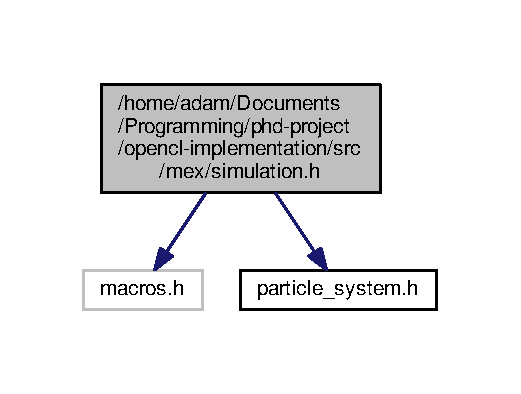
\includegraphics[width=250pt]{simulation_8h__incl}
\end{center}
\end{figure}
\subsection*{Functions}
\begin{DoxyCompactItemize}
\item 
void \hyperlink{simulation_8h_aeb2624c7a86b765725fd80cd426e147d}{increment} ()
\item 
void \hyperlink{simulation_8h_af998f1201f6ff5160003144e5818b8ba}{decrement} ()
\end{DoxyCompactItemize}


\subsection{Function Documentation}
\hypertarget{simulation_8h_af998f1201f6ff5160003144e5818b8ba}{}\index{simulation.\+h@{simulation.\+h}!decrement@{decrement}}
\index{decrement@{decrement}!simulation.\+h@{simulation.\+h}}
\subsubsection[{decrement}]{\setlength{\rightskip}{0pt plus 5cm}void decrement (
\begin{DoxyParamCaption}
{}
\end{DoxyParamCaption}
)}\label{simulation_8h_af998f1201f6ff5160003144e5818b8ba}
\hypertarget{simulation_8h_aeb2624c7a86b765725fd80cd426e147d}{}\index{simulation.\+h@{simulation.\+h}!increment@{increment}}
\index{increment@{increment}!simulation.\+h@{simulation.\+h}}
\subsubsection[{increment}]{\setlength{\rightskip}{0pt plus 5cm}void increment (
\begin{DoxyParamCaption}
{}
\end{DoxyParamCaption}
)}\label{simulation_8h_aeb2624c7a86b765725fd80cd426e147d}

\hypertarget{solid_8h}{}\section{/home/adam/\+Documents/\+Programming/phd-\/project/opencl-\/implementation/src/mex/solid.h File Reference}
\label{solid_8h}\index{/home/adam/\+Documents/\+Programming/phd-\/project/opencl-\/implementation/src/mex/solid.\+h@{/home/adam/\+Documents/\+Programming/phd-\/project/opencl-\/implementation/src/mex/solid.\+h}}
{\ttfamily \#include \char`\"{}particle\+\_\+system.\+h\char`\"{}}\\*
Include dependency graph for solid.\+h\+:
\nopagebreak
\begin{figure}[H]
\begin{center}
\leavevmode
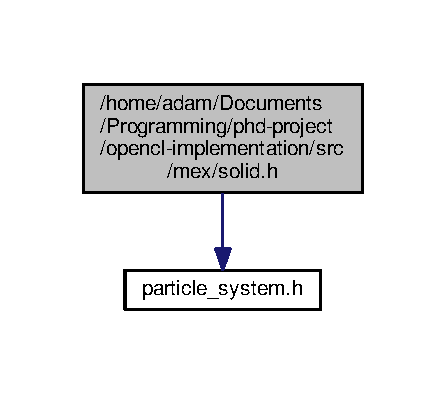
\includegraphics[width=214pt]{solid_8h__incl}
\end{center}
\end{figure}
\subsection*{Data Structures}
\begin{DoxyCompactItemize}
\item 
class \hyperlink{classSolid}{Solid}
\end{DoxyCompactItemize}

\hypertarget{testentry_8c}{}\section{/home/adam/\+Documents/\+Programming/phd-\/project/opencl-\/implementation/src/mex/testentry.c File Reference}
\label{testentry_8c}\index{/home/adam/\+Documents/\+Programming/phd-\/project/opencl-\/implementation/src/mex/testentry.\+c@{/home/adam/\+Documents/\+Programming/phd-\/project/opencl-\/implementation/src/mex/testentry.\+c}}
{\ttfamily \#include $<$assert.\+h$>$}\\*
{\ttfamily \#include $<$string.\+h$>$}\\*
{\ttfamily \#include \char`\"{}mex.\+h\char`\"{}}\\*
{\ttfamily \#include \char`\"{}../note.\+h\char`\"{}}\\*
{\ttfamily \#include \char`\"{}../particle\+\_\+system.\+h\char`\"{}}\\*
{\ttfamily \#include \char`\"{}../opencl/particle\+\_\+system\+\_\+host.\+h\char`\"{}}\\*
Include dependency graph for testentry.\+c\+:
\nopagebreak
\begin{figure}[H]
\begin{center}
\leavevmode
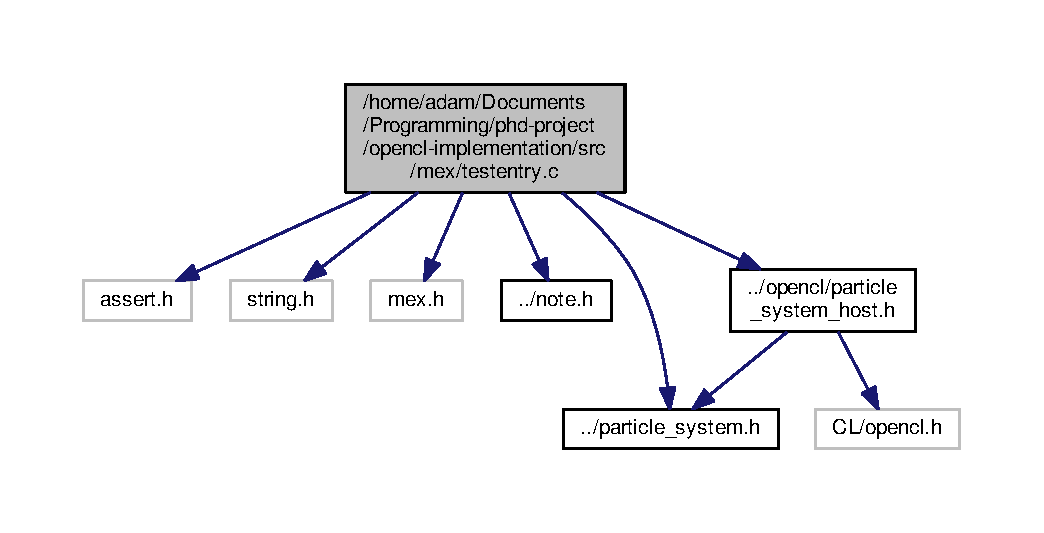
\includegraphics[width=350pt]{testentry_8c__incl}
\end{center}
\end{figure}
\subsection*{Functions}
\begin{DoxyCompactItemize}
\item 
void \hyperlink{testentry_8c_af7dcec3988ba4d873f365b75373e5b09}{on\+Exit} ()
\item 
void \hyperlink{testentry_8c_a6a215cbfde54f82a3ce599228fc3fce5}{mex\+Function} (int nlhs, mx\+Array $\ast$plhs\mbox{[}$\,$\mbox{]}, int nrhs, const mx\+Array $\ast$prhs\mbox{[}$\,$\mbox{]})
\end{DoxyCompactItemize}


\subsection{Function Documentation}
\hypertarget{testentry_8c_a6a215cbfde54f82a3ce599228fc3fce5}{}\index{testentry.\+c@{testentry.\+c}!mex\+Function@{mex\+Function}}
\index{mex\+Function@{mex\+Function}!testentry.\+c@{testentry.\+c}}
\subsubsection[{mex\+Function}]{\setlength{\rightskip}{0pt plus 5cm}void mex\+Function (
\begin{DoxyParamCaption}
\item[{int}]{nlhs, }
\item[{mx\+Array $\ast$}]{plhs\mbox{[}$\,$\mbox{]}, }
\item[{int}]{nrhs, }
\item[{const mx\+Array $\ast$}]{prhs\mbox{[}$\,$\mbox{]}}
\end{DoxyParamCaption}
)}\label{testentry_8c_a6a215cbfde54f82a3ce599228fc3fce5}
\hypertarget{testentry_8c_af7dcec3988ba4d873f365b75373e5b09}{}\index{testentry.\+c@{testentry.\+c}!on\+Exit@{on\+Exit}}
\index{on\+Exit@{on\+Exit}!testentry.\+c@{testentry.\+c}}
\subsubsection[{on\+Exit}]{\setlength{\rightskip}{0pt plus 5cm}void on\+Exit (
\begin{DoxyParamCaption}
{}
\end{DoxyParamCaption}
)}\label{testentry_8c_af7dcec3988ba4d873f365b75373e5b09}

\hypertarget{testentry2_8c}{}\section{/home/adam/\+Documents/\+Programming/phd-\/project/opencl-\/implementation/src/mex/testentry2.c File Reference}
\label{testentry2_8c}\index{/home/adam/\+Documents/\+Programming/phd-\/project/opencl-\/implementation/src/mex/testentry2.\+c@{/home/adam/\+Documents/\+Programming/phd-\/project/opencl-\/implementation/src/mex/testentry2.\+c}}
{\ttfamily \#include \char`\"{}mex.\+h\char`\"{}}\\*
{\ttfamily \#include \char`\"{}../particle\+\_\+system.\+h\char`\"{}}\\*
Include dependency graph for testentry2.\+c\+:
\nopagebreak
\begin{figure}[H]
\begin{center}
\leavevmode
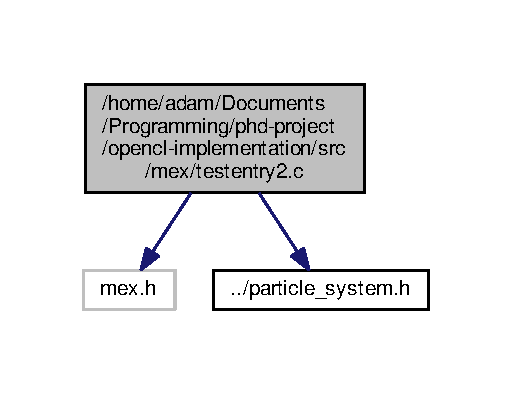
\includegraphics[width=246pt]{testentry2_8c__incl}
\end{center}
\end{figure}
\subsection*{Functions}
\begin{DoxyCompactItemize}
\item 
void \hyperlink{testentry2_8c_af7dcec3988ba4d873f365b75373e5b09}{on\+Exit} ()
\item 
void \hyperlink{testentry2_8c_a6a215cbfde54f82a3ce599228fc3fce5}{mex\+Function} (int nlhs, mx\+Array $\ast$plhs\mbox{[}$\,$\mbox{]}, int nrhs, const mx\+Array $\ast$prhs\mbox{[}$\,$\mbox{]})
\end{DoxyCompactItemize}


\subsection{Function Documentation}
\hypertarget{testentry2_8c_a6a215cbfde54f82a3ce599228fc3fce5}{}\index{testentry2.\+c@{testentry2.\+c}!mex\+Function@{mex\+Function}}
\index{mex\+Function@{mex\+Function}!testentry2.\+c@{testentry2.\+c}}
\subsubsection[{mex\+Function}]{\setlength{\rightskip}{0pt plus 5cm}void mex\+Function (
\begin{DoxyParamCaption}
\item[{int}]{nlhs, }
\item[{mx\+Array $\ast$}]{plhs\mbox{[}$\,$\mbox{]}, }
\item[{int}]{nrhs, }
\item[{const mx\+Array $\ast$}]{prhs\mbox{[}$\,$\mbox{]}}
\end{DoxyParamCaption}
)}\label{testentry2_8c_a6a215cbfde54f82a3ce599228fc3fce5}
\hypertarget{testentry2_8c_af7dcec3988ba4d873f365b75373e5b09}{}\index{testentry2.\+c@{testentry2.\+c}!on\+Exit@{on\+Exit}}
\index{on\+Exit@{on\+Exit}!testentry2.\+c@{testentry2.\+c}}
\subsubsection[{on\+Exit}]{\setlength{\rightskip}{0pt plus 5cm}void on\+Exit (
\begin{DoxyParamCaption}
{}
\end{DoxyParamCaption}
)}\label{testentry2_8c_af7dcec3988ba4d873f365b75373e5b09}

\hypertarget{testentry__wrap_8m}{}\section{/home/adam/\+Documents/\+Programming/phd-\/project/opencl-\/implementation/src/mex/testentry\+\_\+wrap.m File Reference}
\label{testentry__wrap_8m}\index{/home/adam/\+Documents/\+Programming/phd-\/project/opencl-\/implementation/src/mex/testentry\+\_\+wrap.\+m@{/home/adam/\+Documents/\+Programming/phd-\/project/opencl-\/implementation/src/mex/testentry\+\_\+wrap.\+m}}
\subsection*{Functions}
\begin{DoxyCompactItemize}
\item 
\hyperlink{testentry__wrap_8m_a5bba147329d5e8aefcc9d9f95694ddcf}{setenv} (\textquotesingle{}E\+X\+E\+\_\+\+P\+A\+T\+H\textquotesingle{}, \hyperlink{testentry__wrap_8m_a423dea0fe67e3aae03e74bd726f484b4}{entrypath})
\end{DoxyCompactItemize}
\subsection*{Variables}
\begin{DoxyCompactItemize}
\item 
function \hyperlink{testentry__wrap_8m_a4124bc0a9335c27f086f24ba207a4912}{a}
\item 
\hyperlink{testentry__wrap_8m_a423dea0fe67e3aae03e74bd726f484b4}{entrypath} = fileparts(entrypath)
\end{DoxyCompactItemize}


\subsection{Function Documentation}
\hypertarget{testentry__wrap_8m_a5bba147329d5e8aefcc9d9f95694ddcf}{}\index{testentry\+\_\+wrap.\+m@{testentry\+\_\+wrap.\+m}!setenv@{setenv}}
\index{setenv@{setenv}!testentry\+\_\+wrap.\+m@{testentry\+\_\+wrap.\+m}}
\subsubsection[{setenv}]{\setlength{\rightskip}{0pt plus 5cm}setenv (
\begin{DoxyParamCaption}
\item[{\textquotesingle{}E\+X\+E\+\_\+\+P\+A\+T\+H\textquotesingle{}}]{, }
\item[{{\bf entrypath}}]{}
\end{DoxyParamCaption}
)}\label{testentry__wrap_8m_a5bba147329d5e8aefcc9d9f95694ddcf}


\subsection{Variable Documentation}
\hypertarget{testentry__wrap_8m_a4124bc0a9335c27f086f24ba207a4912}{}\index{testentry\+\_\+wrap.\+m@{testentry\+\_\+wrap.\+m}!a@{a}}
\index{a@{a}!testentry\+\_\+wrap.\+m@{testentry\+\_\+wrap.\+m}}
\subsubsection[{a}]{\setlength{\rightskip}{0pt plus 5cm}a}\label{testentry__wrap_8m_a4124bc0a9335c27f086f24ba207a4912}
{\bfseries Initial value\+:}
\begin{DoxyCode}
= testentry\_wrap()

\hyperlink{testentry__wrap_8m_a423dea0fe67e3aae03e74bd726f484b4}{entrypath} = which('testentry')
\end{DoxyCode}
\hypertarget{testentry__wrap_8m_a423dea0fe67e3aae03e74bd726f484b4}{}\index{testentry\+\_\+wrap.\+m@{testentry\+\_\+wrap.\+m}!entrypath@{entrypath}}
\index{entrypath@{entrypath}!testentry\+\_\+wrap.\+m@{testentry\+\_\+wrap.\+m}}
\subsubsection[{entrypath}]{\setlength{\rightskip}{0pt plus 5cm}entrypath = fileparts(entrypath)}\label{testentry__wrap_8m_a423dea0fe67e3aae03e74bd726f484b4}

\hypertarget{testmex_8c}{}\section{/home/adam/\+Documents/\+Programming/phd-\/project/opencl-\/implementation/src/mex/testmex.c File Reference}
\label{testmex_8c}\index{/home/adam/\+Documents/\+Programming/phd-\/project/opencl-\/implementation/src/mex/testmex.\+c@{/home/adam/\+Documents/\+Programming/phd-\/project/opencl-\/implementation/src/mex/testmex.\+c}}
{\ttfamily \#include \char`\"{}mex.\+h\char`\"{}}\\*
{\ttfamily \#include $<$cmath$>$}\\*
{\ttfamily \#include $<$cstring$>$}\\*
Include dependency graph for testmex.\+c\+:
\nopagebreak
\begin{figure}[H]
\begin{center}
\leavevmode
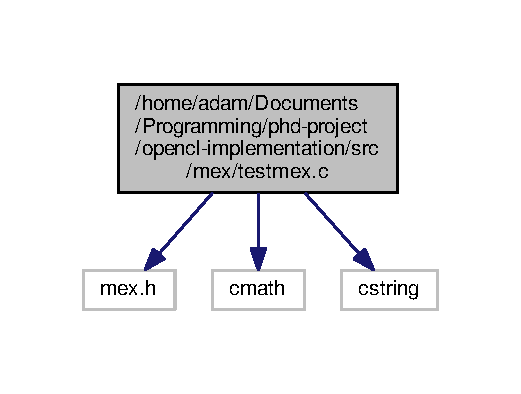
\includegraphics[width=250pt]{testmex_8c__incl}
\end{center}
\end{figure}
\subsection*{Functions}
\begin{DoxyCompactItemize}
\item 
void \hyperlink{testmex_8c_a6a215cbfde54f82a3ce599228fc3fce5}{mex\+Function} (int nlhs, mx\+Array $\ast$plhs\mbox{[}$\,$\mbox{]}, int nrhs, const mx\+Array $\ast$prhs\mbox{[}$\,$\mbox{]})
\end{DoxyCompactItemize}


\subsection{Function Documentation}
\hypertarget{testmex_8c_a6a215cbfde54f82a3ce599228fc3fce5}{}\index{testmex.\+c@{testmex.\+c}!mex\+Function@{mex\+Function}}
\index{mex\+Function@{mex\+Function}!testmex.\+c@{testmex.\+c}}
\subsubsection[{mex\+Function}]{\setlength{\rightskip}{0pt plus 5cm}void mex\+Function (
\begin{DoxyParamCaption}
\item[{int}]{nlhs, }
\item[{mx\+Array $\ast$}]{plhs\mbox{[}$\,$\mbox{]}, }
\item[{int}]{nrhs, }
\item[{const mx\+Array $\ast$}]{prhs\mbox{[}$\,$\mbox{]}}
\end{DoxyParamCaption}
)}\label{testmex_8c_a6a215cbfde54f82a3ce599228fc3fce5}

\hypertarget{mex_2testopencl_8c}{}\section{/home/adam/\+Documents/\+Programming/phd-\/project/opencl-\/implementation/src/mex/testopencl.c File Reference}
\label{mex_2testopencl_8c}\index{/home/adam/\+Documents/\+Programming/phd-\/project/opencl-\/implementation/src/mex/testopencl.\+c@{/home/adam/\+Documents/\+Programming/phd-\/project/opencl-\/implementation/src/mex/testopencl.\+c}}
{\ttfamily \#include \char`\"{}../opencl/particle\+\_\+system\+\_\+host.\+h\char`\"{}}\\*
{\ttfamily \#include \char`\"{}mex.\+h\char`\"{}}\\*
Include dependency graph for testopencl.\+c\+:
\nopagebreak
\begin{figure}[H]
\begin{center}
\leavevmode
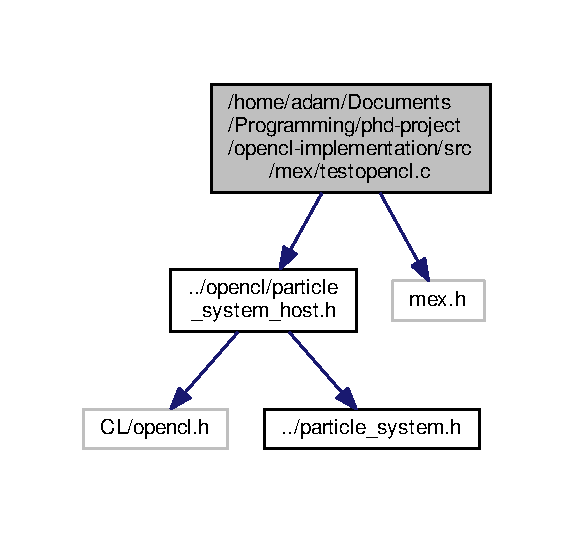
\includegraphics[width=276pt]{mex_2testopencl_8c__incl}
\end{center}
\end{figure}
\subsection*{Functions}
\begin{DoxyCompactItemize}
\item 
void \hyperlink{mex_2testopencl_8c_a6a215cbfde54f82a3ce599228fc3fce5}{mex\+Function} (int nlhs, mx\+Array $\ast$plhs\mbox{[}$\,$\mbox{]}, int nrhs, const mx\+Array $\ast$prhs\mbox{[}$\,$\mbox{]})
\end{DoxyCompactItemize}


\subsection{Function Documentation}
\hypertarget{mex_2testopencl_8c_a6a215cbfde54f82a3ce599228fc3fce5}{}\index{mex/testopencl.\+c@{mex/testopencl.\+c}!mex\+Function@{mex\+Function}}
\index{mex\+Function@{mex\+Function}!mex/testopencl.\+c@{mex/testopencl.\+c}}
\subsubsection[{mex\+Function}]{\setlength{\rightskip}{0pt plus 5cm}void mex\+Function (
\begin{DoxyParamCaption}
\item[{int}]{nlhs, }
\item[{mx\+Array $\ast$}]{plhs\mbox{[}$\,$\mbox{]}, }
\item[{int}]{nrhs, }
\item[{const mx\+Array $\ast$}]{prhs\mbox{[}$\,$\mbox{]}}
\end{DoxyParamCaption}
)}\label{mex_2testopencl_8c_a6a215cbfde54f82a3ce599228fc3fce5}

\hypertarget{testopencl_8c}{}\section{/home/adam/\+Documents/\+Programming/phd-\/project/opencl-\/implementation/src/testopencl.c File Reference}
\label{testopencl_8c}\index{/home/adam/\+Documents/\+Programming/phd-\/project/opencl-\/implementation/src/testopencl.\+c@{/home/adam/\+Documents/\+Programming/phd-\/project/opencl-\/implementation/src/testopencl.\+c}}
{\ttfamily \#include $<$assert.\+h$>$}\\*
{\ttfamily \#include $<$stdio.\+h$>$}\\*
{\ttfamily \#include \char`\"{}note.\+h\char`\"{}}\\*
{\ttfamily \#include \char`\"{}particle\+\_\+system.\+h\char`\"{}}\\*
{\ttfamily \#include \char`\"{}opencl/particle\+\_\+system\+\_\+host.\+h\char`\"{}}\\*
Include dependency graph for testopencl.\+c\+:
\nopagebreak
\begin{figure}[H]
\begin{center}
\leavevmode
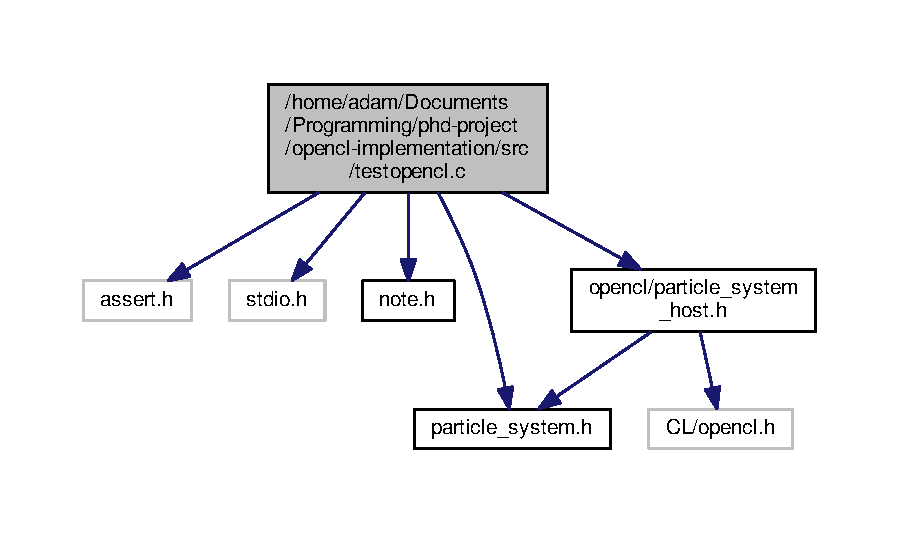
\includegraphics[width=350pt]{testopencl_8c__incl}
\end{center}
\end{figure}
\subsection*{Functions}
\begin{DoxyCompactItemize}
\item 
int \hyperlink{testopencl_8c_ae66f6b31b5ad750f1fe042a706a4e3d4}{main} ()
\end{DoxyCompactItemize}


\subsection{Function Documentation}
\hypertarget{testopencl_8c_ae66f6b31b5ad750f1fe042a706a4e3d4}{}\index{testopencl.\+c@{testopencl.\+c}!main@{main}}
\index{main@{main}!testopencl.\+c@{testopencl.\+c}}
\subsubsection[{main}]{\setlength{\rightskip}{0pt plus 5cm}int main (
\begin{DoxyParamCaption}
{}
\end{DoxyParamCaption}
)}\label{testopencl_8c_ae66f6b31b5ad750f1fe042a706a4e3d4}

\hypertarget{note_8c}{}\section{/home/adam/\+Documents/\+Programming/phd-\/project/opencl-\/implementation/src/note.c File Reference}
\label{note_8c}\index{/home/adam/\+Documents/\+Programming/phd-\/project/opencl-\/implementation/src/note.\+c@{/home/adam/\+Documents/\+Programming/phd-\/project/opencl-\/implementation/src/note.\+c}}
{\ttfamily \#include $<$stdio.\+h$>$}\\*
{\ttfamily \#include $<$stdarg.\+h$>$}\\*
Include dependency graph for note.\+c\+:
\nopagebreak
\begin{figure}[H]
\begin{center}
\leavevmode
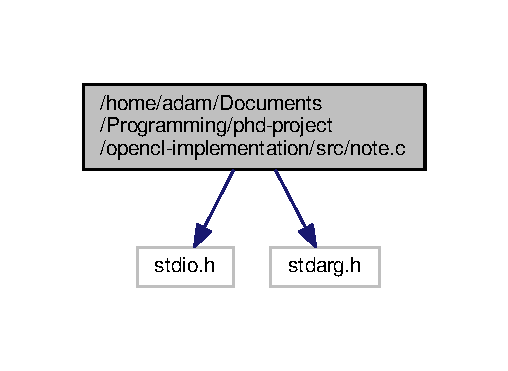
\includegraphics[width=244pt]{note_8c__incl}
\end{center}
\end{figure}
\subsection*{Functions}
\begin{DoxyCompactItemize}
\item 
void \hyperlink{note_8c_a7ea7d156d3e967ee01abe023c8e0c801}{set\+\_\+log\+\_\+level} (unsigned int loglevel)
\item 
void \hyperlink{note_8c_a48c08718596a327e8dd9f9975c751426}{note} (unsigned int level, const char $\ast$fmt,...)
\end{DoxyCompactItemize}


\subsection{Function Documentation}
\hypertarget{note_8c_a48c08718596a327e8dd9f9975c751426}{}\index{note.\+c@{note.\+c}!note@{note}}
\index{note@{note}!note.\+c@{note.\+c}}
\subsubsection[{note}]{\setlength{\rightskip}{0pt plus 5cm}void note (
\begin{DoxyParamCaption}
\item[{unsigned int}]{level, }
\item[{const char $\ast$}]{fmt, }
\item[{}]{...}
\end{DoxyParamCaption}
)}\label{note_8c_a48c08718596a327e8dd9f9975c751426}
\hypertarget{note_8c_a7ea7d156d3e967ee01abe023c8e0c801}{}\index{note.\+c@{note.\+c}!set\+\_\+log\+\_\+level@{set\+\_\+log\+\_\+level}}
\index{set\+\_\+log\+\_\+level@{set\+\_\+log\+\_\+level}!note.\+c@{note.\+c}}
\subsubsection[{set\+\_\+log\+\_\+level}]{\setlength{\rightskip}{0pt plus 5cm}void set\+\_\+log\+\_\+level (
\begin{DoxyParamCaption}
\item[{unsigned int}]{loglevel}
\end{DoxyParamCaption}
)}\label{note_8c_a7ea7d156d3e967ee01abe023c8e0c801}

\hypertarget{note_8h}{}\section{/home/adam/\+Documents/\+Programming/phd-\/project/opencl-\/implementation/src/note.h File Reference}
\label{note_8h}\index{/home/adam/\+Documents/\+Programming/phd-\/project/opencl-\/implementation/src/note.\+h@{/home/adam/\+Documents/\+Programming/phd-\/project/opencl-\/implementation/src/note.\+h}}
This graph shows which files directly or indirectly include this file\+:
\nopagebreak
\begin{figure}[H]
\begin{center}
\leavevmode
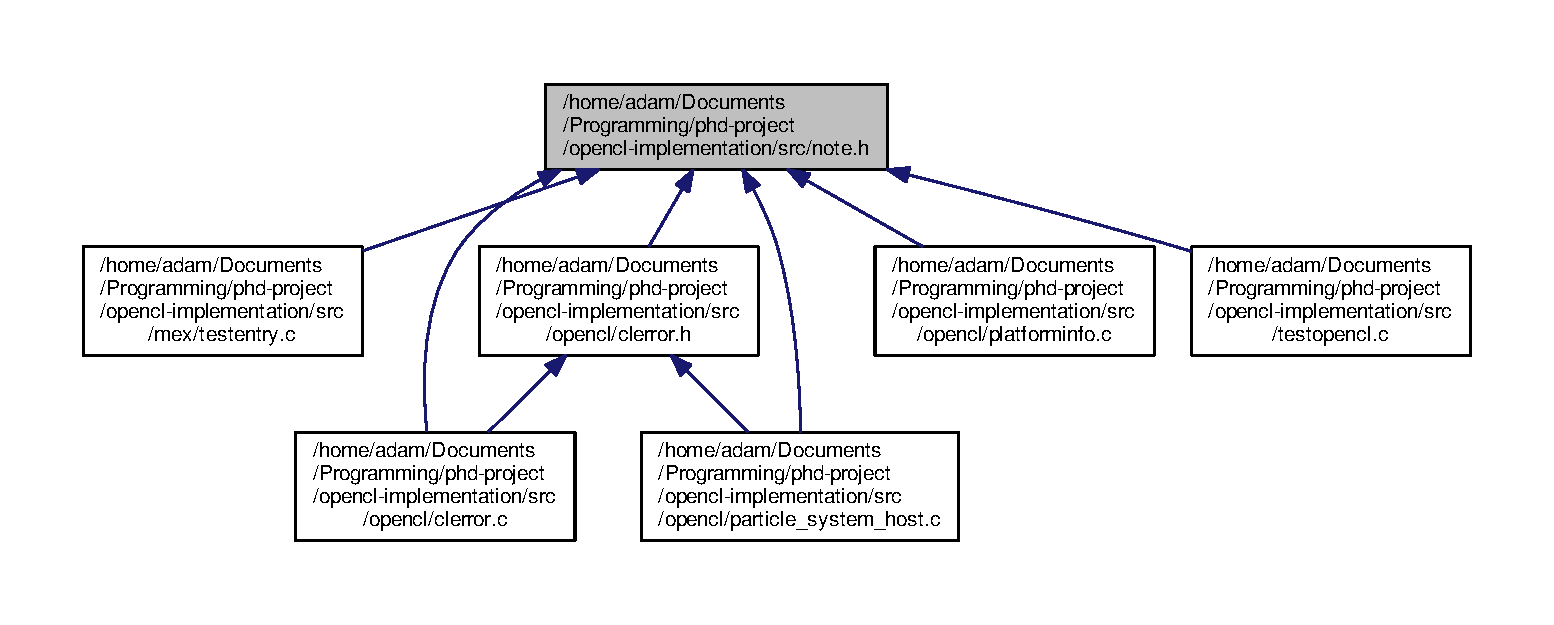
\includegraphics[width=350pt]{note_8h__dep__incl}
\end{center}
\end{figure}
\subsection*{Functions}
\begin{DoxyCompactItemize}
\item 
void \hyperlink{note_8h_a7ea7d156d3e967ee01abe023c8e0c801}{set\+\_\+log\+\_\+level} (unsigned int loglevel)
\item 
void \hyperlink{note_8h_a48c08718596a327e8dd9f9975c751426}{note} (unsigned int level, const char $\ast$fmt,...)
\end{DoxyCompactItemize}


\subsection{Function Documentation}
\hypertarget{note_8h_a48c08718596a327e8dd9f9975c751426}{}\index{note.\+h@{note.\+h}!note@{note}}
\index{note@{note}!note.\+h@{note.\+h}}
\subsubsection[{note}]{\setlength{\rightskip}{0pt plus 5cm}void note (
\begin{DoxyParamCaption}
\item[{unsigned int}]{level, }
\item[{const char $\ast$}]{fmt, }
\item[{}]{...}
\end{DoxyParamCaption}
)}\label{note_8h_a48c08718596a327e8dd9f9975c751426}
\hypertarget{note_8h_a7ea7d156d3e967ee01abe023c8e0c801}{}\index{note.\+h@{note.\+h}!set\+\_\+log\+\_\+level@{set\+\_\+log\+\_\+level}}
\index{set\+\_\+log\+\_\+level@{set\+\_\+log\+\_\+level}!note.\+h@{note.\+h}}
\subsubsection[{set\+\_\+log\+\_\+level}]{\setlength{\rightskip}{0pt plus 5cm}void set\+\_\+log\+\_\+level (
\begin{DoxyParamCaption}
\item[{unsigned int}]{loglevel}
\end{DoxyParamCaption}
)}\label{note_8h_a7ea7d156d3e967ee01abe023c8e0c801}

\hypertarget{clerror_8c}{}\section{/home/adam/\+Documents/\+Programming/phd-\/project/opencl-\/implementation/src/opencl/clerror.c File Reference}
\label{clerror_8c}\index{/home/adam/\+Documents/\+Programming/phd-\/project/opencl-\/implementation/src/opencl/clerror.\+c@{/home/adam/\+Documents/\+Programming/phd-\/project/opencl-\/implementation/src/opencl/clerror.\+c}}
{\ttfamily \#include \char`\"{}clerror.\+h\char`\"{}}\\*
{\ttfamily \#include \char`\"{}../note.\+h\char`\"{}}\\*
Include dependency graph for clerror.\+c\+:
\nopagebreak
\begin{figure}[H]
\begin{center}
\leavevmode
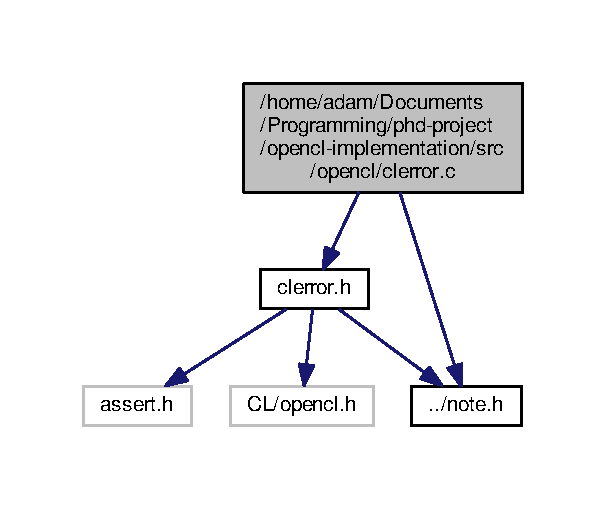
\includegraphics[width=291pt]{clerror_8c__incl}
\end{center}
\end{figure}
\subsection*{Functions}
\begin{DoxyCompactItemize}
\item 
void \hyperlink{clerror_8c_a940ebbff9ed6d229736b68331aff4081}{print\+C\+L\+Error} (cl\+\_\+int error)
\item 
void \hyperlink{clerror_8c_ac38d1b2a2242ccbb27a8dd94f4e61d85}{context\+Error\+Callback} (const char $\ast$errinfo, const void $\ast$private\+\_\+info, size\+\_\+t cb, void $\ast$user\+\_\+data)
\end{DoxyCompactItemize}


\subsection{Function Documentation}
\hypertarget{clerror_8c_ac38d1b2a2242ccbb27a8dd94f4e61d85}{}\index{clerror.\+c@{clerror.\+c}!context\+Error\+Callback@{context\+Error\+Callback}}
\index{context\+Error\+Callback@{context\+Error\+Callback}!clerror.\+c@{clerror.\+c}}
\subsubsection[{context\+Error\+Callback}]{\setlength{\rightskip}{0pt plus 5cm}void context\+Error\+Callback (
\begin{DoxyParamCaption}
\item[{const char $\ast$}]{errinfo, }
\item[{const void $\ast$}]{private\+\_\+info, }
\item[{size\+\_\+t}]{cb, }
\item[{void $\ast$}]{user\+\_\+data}
\end{DoxyParamCaption}
)}\label{clerror_8c_ac38d1b2a2242ccbb27a8dd94f4e61d85}
\hypertarget{clerror_8c_a940ebbff9ed6d229736b68331aff4081}{}\index{clerror.\+c@{clerror.\+c}!print\+C\+L\+Error@{print\+C\+L\+Error}}
\index{print\+C\+L\+Error@{print\+C\+L\+Error}!clerror.\+c@{clerror.\+c}}
\subsubsection[{print\+C\+L\+Error}]{\setlength{\rightskip}{0pt plus 5cm}void print\+C\+L\+Error (
\begin{DoxyParamCaption}
\item[{cl\+\_\+int}]{error}
\end{DoxyParamCaption}
)}\label{clerror_8c_a940ebbff9ed6d229736b68331aff4081}

\hypertarget{clerror_8h}{}\section{/home/adam/\+Documents/\+Programming/phd-\/project/opencl-\/implementation/src/opencl/clerror.h File Reference}
\label{clerror_8h}\index{/home/adam/\+Documents/\+Programming/phd-\/project/opencl-\/implementation/src/opencl/clerror.\+h@{/home/adam/\+Documents/\+Programming/phd-\/project/opencl-\/implementation/src/opencl/clerror.\+h}}
{\ttfamily \#include $<$assert.\+h$>$}\\*
{\ttfamily \#include $<$C\+L/opencl.\+h$>$}\\*
{\ttfamily \#include \char`\"{}../note.\+h\char`\"{}}\\*
Include dependency graph for clerror.\+h\+:
\nopagebreak
\begin{figure}[H]
\begin{center}
\leavevmode
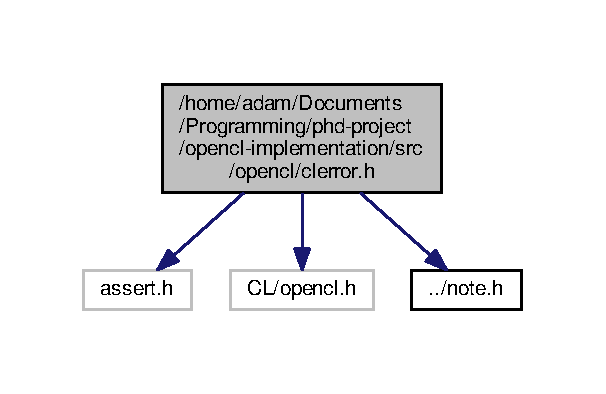
\includegraphics[width=291pt]{clerror_8h__incl}
\end{center}
\end{figure}
This graph shows which files directly or indirectly include this file\+:
\nopagebreak
\begin{figure}[H]
\begin{center}
\leavevmode
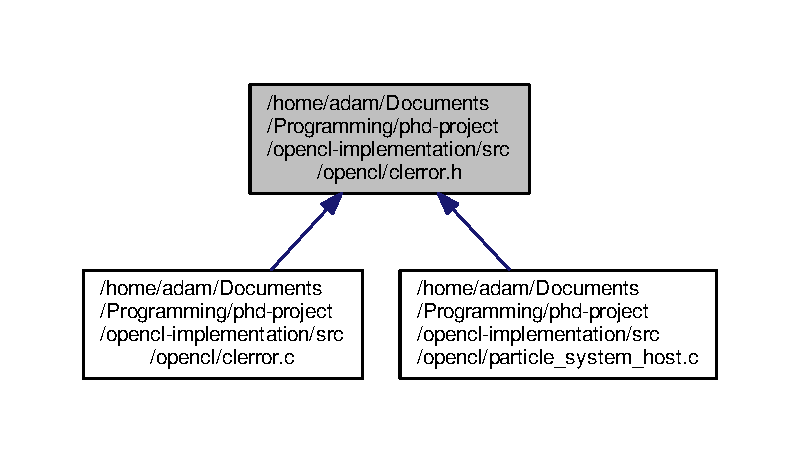
\includegraphics[width=350pt]{clerror_8h__dep__incl}
\end{center}
\end{figure}
\subsection*{Macros}
\begin{DoxyCompactItemize}
\item 
\#define \hyperlink{clerror_8h_aca68c0d4ac8df0838e209fb5300f7be3}{A\+S\+S\+E\+R\+T}(x)~assert(x)
\item 
\#define \hyperlink{clerror_8h_a40f17fa8e1e5f1faeb622385348fe469}{H\+A\+N\+D\+L\+E\+\_\+\+C\+L\+\_\+\+E\+R\+R\+O\+R}(x)~\{ \hyperlink{note_8h_a48c08718596a327e8dd9f9975c751426}{note}(0, \#x\char`\"{}\textbackslash{}n\char`\"{}); cl\+\_\+int e = x; if (e != C\+L\+\_\+\+S\+U\+C\+C\+E\+S\+S) \hyperlink{clerror_8h_a940ebbff9ed6d229736b68331aff4081}{print\+C\+L\+Error}(e); \hyperlink{clerror_8h_aca68c0d4ac8df0838e209fb5300f7be3}{A\+S\+S\+E\+R\+T}(e == C\+L\+\_\+\+S\+U\+C\+C\+E\+S\+S); \}
\end{DoxyCompactItemize}
\subsection*{Functions}
\begin{DoxyCompactItemize}
\item 
void \hyperlink{clerror_8h_a940ebbff9ed6d229736b68331aff4081}{print\+C\+L\+Error} (cl\+\_\+int error)
\item 
void \hyperlink{clerror_8h_ac38d1b2a2242ccbb27a8dd94f4e61d85}{context\+Error\+Callback} (const char $\ast$errinfo, const void $\ast$private\+\_\+info, size\+\_\+t cb, void $\ast$user\+\_\+data)
\end{DoxyCompactItemize}


\subsection{Macro Definition Documentation}
\hypertarget{clerror_8h_aca68c0d4ac8df0838e209fb5300f7be3}{}\index{clerror.\+h@{clerror.\+h}!A\+S\+S\+E\+R\+T@{A\+S\+S\+E\+R\+T}}
\index{A\+S\+S\+E\+R\+T@{A\+S\+S\+E\+R\+T}!clerror.\+h@{clerror.\+h}}
\subsubsection[{A\+S\+S\+E\+R\+T}]{\setlength{\rightskip}{0pt plus 5cm}\#define A\+S\+S\+E\+R\+T(
\begin{DoxyParamCaption}
\item[{}]{x}
\end{DoxyParamCaption}
)~assert(x)}\label{clerror_8h_aca68c0d4ac8df0838e209fb5300f7be3}
\hypertarget{clerror_8h_a40f17fa8e1e5f1faeb622385348fe469}{}\index{clerror.\+h@{clerror.\+h}!H\+A\+N\+D\+L\+E\+\_\+\+C\+L\+\_\+\+E\+R\+R\+O\+R@{H\+A\+N\+D\+L\+E\+\_\+\+C\+L\+\_\+\+E\+R\+R\+O\+R}}
\index{H\+A\+N\+D\+L\+E\+\_\+\+C\+L\+\_\+\+E\+R\+R\+O\+R@{H\+A\+N\+D\+L\+E\+\_\+\+C\+L\+\_\+\+E\+R\+R\+O\+R}!clerror.\+h@{clerror.\+h}}
\subsubsection[{H\+A\+N\+D\+L\+E\+\_\+\+C\+L\+\_\+\+E\+R\+R\+O\+R}]{\setlength{\rightskip}{0pt plus 5cm}\#define H\+A\+N\+D\+L\+E\+\_\+\+C\+L\+\_\+\+E\+R\+R\+O\+R(
\begin{DoxyParamCaption}
\item[{}]{x}
\end{DoxyParamCaption}
)~\{ {\bf note}(0, \#x\char`\"{}\textbackslash{}n\char`\"{}); cl\+\_\+int e = x; if (e != C\+L\+\_\+\+S\+U\+C\+C\+E\+S\+S) {\bf print\+C\+L\+Error}(e); {\bf A\+S\+S\+E\+R\+T}(e == C\+L\+\_\+\+S\+U\+C\+C\+E\+S\+S); \}}\label{clerror_8h_a40f17fa8e1e5f1faeb622385348fe469}


\subsection{Function Documentation}
\hypertarget{clerror_8h_ac38d1b2a2242ccbb27a8dd94f4e61d85}{}\index{clerror.\+h@{clerror.\+h}!context\+Error\+Callback@{context\+Error\+Callback}}
\index{context\+Error\+Callback@{context\+Error\+Callback}!clerror.\+h@{clerror.\+h}}
\subsubsection[{context\+Error\+Callback}]{\setlength{\rightskip}{0pt plus 5cm}void context\+Error\+Callback (
\begin{DoxyParamCaption}
\item[{const char $\ast$}]{errinfo, }
\item[{const void $\ast$}]{private\+\_\+info, }
\item[{size\+\_\+t}]{cb, }
\item[{void $\ast$}]{user\+\_\+data}
\end{DoxyParamCaption}
)}\label{clerror_8h_ac38d1b2a2242ccbb27a8dd94f4e61d85}
\hypertarget{clerror_8h_a940ebbff9ed6d229736b68331aff4081}{}\index{clerror.\+h@{clerror.\+h}!print\+C\+L\+Error@{print\+C\+L\+Error}}
\index{print\+C\+L\+Error@{print\+C\+L\+Error}!clerror.\+h@{clerror.\+h}}
\subsubsection[{print\+C\+L\+Error}]{\setlength{\rightskip}{0pt plus 5cm}void print\+C\+L\+Error (
\begin{DoxyParamCaption}
\item[{cl\+\_\+int}]{error}
\end{DoxyParamCaption}
)}\label{clerror_8h_a940ebbff9ed6d229736b68331aff4081}

\hypertarget{particle__system__host_8c}{}\section{/home/adam/\+Documents/\+Programming/phd-\/project/opencl-\/implementation/src/opencl/particle\+\_\+system\+\_\+host.c File Reference}
\label{particle__system__host_8c}\index{/home/adam/\+Documents/\+Programming/phd-\/project/opencl-\/implementation/src/opencl/particle\+\_\+system\+\_\+host.\+c@{/home/adam/\+Documents/\+Programming/phd-\/project/opencl-\/implementation/src/opencl/particle\+\_\+system\+\_\+host.\+c}}
{\ttfamily \#include $<$stdio.\+h$>$}\\*
{\ttfamily \#include $<$stdlib.\+h$>$}\\*
{\ttfamily \#include $<$string.\+h$>$}\\*
{\ttfamily \#include $<$math.\+h$>$}\\*
{\ttfamily \#include $<$C\+L/opencl.\+h$>$}\\*
{\ttfamily \#include \char`\"{}clerror.\+h\char`\"{}}\\*
{\ttfamily \#include \char`\"{}particle\+\_\+system\+\_\+host.\+h\char`\"{}}\\*
{\ttfamily \#include \char`\"{}../particle\+\_\+system.\+h\char`\"{}}\\*
{\ttfamily \#include \char`\"{}../note.\+h\char`\"{}}\\*
{\ttfamily \#include \char`\"{}../3rdparty/whereami.\+h\char`\"{}}\\*
{\ttfamily \#include \char`\"{}platforminfo.\+h\char`\"{}}\\*
Include dependency graph for particle\+\_\+system\+\_\+host.\+c\+:
\nopagebreak
\begin{figure}[H]
\begin{center}
\leavevmode
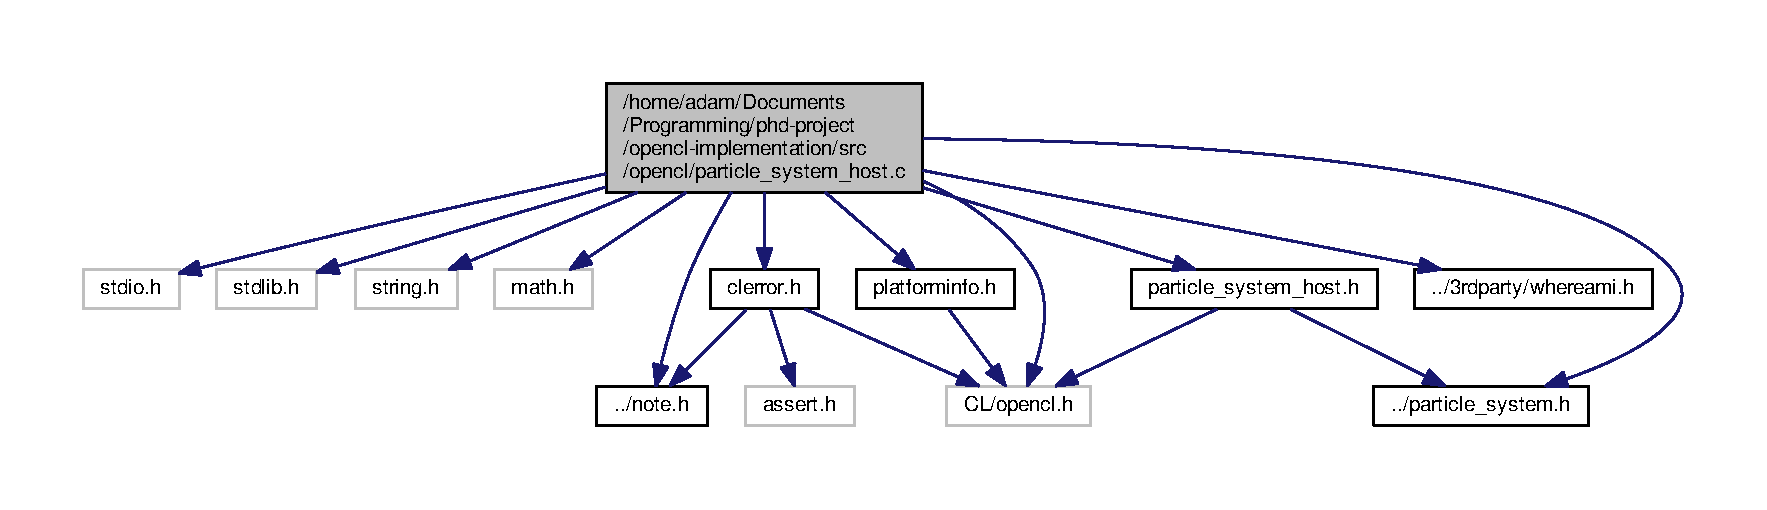
\includegraphics[width=350pt]{particle__system__host_8c__incl}
\end{center}
\end{figure}
\subsection*{Macros}
\begin{DoxyCompactItemize}
\item 
\#define \hyperlink{particle__system__host_8c_a46cb5aeb6a7cf1d2b4390d87d3eb6ab6}{N\+U\+M\+\_\+\+P\+S\+\_\+\+A\+R\+G\+S}~10
\item 
\#define \hyperlink{particle__system__host_8c_aba1cf17d90e669f17aa5c265642d871d}{W\+G\+\_\+\+F\+U\+J\+\_\+\+S\+Z}~896
\end{DoxyCompactItemize}
\subsection*{Functions}
\begin{DoxyCompactItemize}
\item 
void \hyperlink{particle__system__host_8c_a744914e82d7deaaab9366819f7570ace}{init\+\_\+ps\+\_\+opencl} ()
\item 
void \hyperlink{particle__system__host_8c_a913da98edf2caadbdc7e74a2c04a72b9}{increment\+\_\+position\+\_\+0\+\_\+device\+\_\+opencl} ()
\item 
void \hyperlink{particle__system__host_8c_a385a5fd6747f1639c09f17df6791ebd5}{decrement\+\_\+position\+\_\+0\+\_\+device\+\_\+opencl} ()
\item 
void \hyperlink{particle__system__host_8c_a2d2a85cfd370a03d94db3e13b6b1d2e0}{bin\+\_\+and\+\_\+sort\+\_\+device\+\_\+opencl} (\hyperlink{structpsdata}{psdata} $\ast$data)
\item 
void \hyperlink{particle__system__host_8c_a6a8c640dd557b7a19fe506f24f58c2ae}{find\+\_\+particle\+\_\+bins\+\_\+device\+\_\+opencl} (\hyperlink{structpsdata}{psdata} $\ast$data)
\item 
void \hyperlink{particle__system__host_8c_ae135bc768db782f0b315a07b0cf9d61a}{count\+\_\+particles\+\_\+in\+\_\+bins\+\_\+device\+\_\+opencl} (\hyperlink{structpsdata}{psdata} $\ast$data)
\item 
void \hyperlink{particle__system__host_8c_a2f9361e3844559923a7128b5c4770cc9}{populate\+\_\+position\+\_\+cuboid\+\_\+device\+\_\+opencl} (double x1, double y1, double z1, double x2, double y2, double z2, unsigned int xsize, unsigned int ysize, unsigned int zsize)
\item 
\hyperlink{structpsdata__bufList}{psdata\+\_\+buf\+List} \hyperlink{particle__system__host_8c_a2a290247d653a7f0c63f1a9ebc0c300d}{create\+\_\+psdata\+\_\+opencl} (\hyperlink{structpsdata}{psdata} data)
\item 
void \hyperlink{particle__system__host_8c_a264aaddb80e120e5ea4aee8685dc89ed}{opencl\+\_\+use\+\_\+buflist} (\hyperlink{structpsdata__bufList}{psdata\+\_\+buf\+List} bl)
\item 
void \hyperlink{particle__system__host_8c_a12619fd915a64b4a747df1a396a33449}{opencl\+\_\+set\+\_\+kernel\+\_\+buflist} (\hyperlink{structpsdata__bufList}{psdata\+\_\+buf\+List} bl, cl\+\_\+kernel kernel)
\item 
void \hyperlink{particle__system__host_8c_a7cedfb0b69b1ed8eea5ed8504385fdf8}{free\+\_\+psdata\+\_\+opencl} (\hyperlink{structpsdata__bufList}{psdata\+\_\+buf\+List} bl)
\item 
void \hyperlink{particle__system__host_8c_a017aa0e283c0bb6ee128ff69cf10dd81}{sync\+\_\+psdata\+\_\+host\+\_\+to\+\_\+device} (\hyperlink{structpsdata}{psdata} data, \hyperlink{structpsdata__bufList}{psdata\+\_\+buf\+List} bl)
\item 
void \hyperlink{particle__system__host_8c_a543f95a759ce9b341f399c0c7e52b909}{sync\+\_\+psdata\+\_\+device\+\_\+to\+\_\+host} (\hyperlink{structpsdata}{psdata} data, \hyperlink{structpsdata__bufList}{psdata\+\_\+buf\+List} bl)
\item 
void \hyperlink{particle__system__host_8c_ae70d2a7474666f266b0ea73b278989bf}{terminate\+\_\+ps\+\_\+opencl} ()
\end{DoxyCompactItemize}


\subsection{Macro Definition Documentation}
\hypertarget{particle__system__host_8c_a46cb5aeb6a7cf1d2b4390d87d3eb6ab6}{}\index{particle\+\_\+system\+\_\+host.\+c@{particle\+\_\+system\+\_\+host.\+c}!N\+U\+M\+\_\+\+P\+S\+\_\+\+A\+R\+G\+S@{N\+U\+M\+\_\+\+P\+S\+\_\+\+A\+R\+G\+S}}
\index{N\+U\+M\+\_\+\+P\+S\+\_\+\+A\+R\+G\+S@{N\+U\+M\+\_\+\+P\+S\+\_\+\+A\+R\+G\+S}!particle\+\_\+system\+\_\+host.\+c@{particle\+\_\+system\+\_\+host.\+c}}
\subsubsection[{N\+U\+M\+\_\+\+P\+S\+\_\+\+A\+R\+G\+S}]{\setlength{\rightskip}{0pt plus 5cm}\#define N\+U\+M\+\_\+\+P\+S\+\_\+\+A\+R\+G\+S~10}\label{particle__system__host_8c_a46cb5aeb6a7cf1d2b4390d87d3eb6ab6}
\hypertarget{particle__system__host_8c_aba1cf17d90e669f17aa5c265642d871d}{}\index{particle\+\_\+system\+\_\+host.\+c@{particle\+\_\+system\+\_\+host.\+c}!W\+G\+\_\+\+F\+U\+J\+\_\+\+S\+Z@{W\+G\+\_\+\+F\+U\+J\+\_\+\+S\+Z}}
\index{W\+G\+\_\+\+F\+U\+J\+\_\+\+S\+Z@{W\+G\+\_\+\+F\+U\+J\+\_\+\+S\+Z}!particle\+\_\+system\+\_\+host.\+c@{particle\+\_\+system\+\_\+host.\+c}}
\subsubsection[{W\+G\+\_\+\+F\+U\+J\+\_\+\+S\+Z}]{\setlength{\rightskip}{0pt plus 5cm}\#define W\+G\+\_\+\+F\+U\+J\+\_\+\+S\+Z~896}\label{particle__system__host_8c_aba1cf17d90e669f17aa5c265642d871d}


\subsection{Function Documentation}
\hypertarget{particle__system__host_8c_a2d2a85cfd370a03d94db3e13b6b1d2e0}{}\index{particle\+\_\+system\+\_\+host.\+c@{particle\+\_\+system\+\_\+host.\+c}!bin\+\_\+and\+\_\+sort\+\_\+device\+\_\+opencl@{bin\+\_\+and\+\_\+sort\+\_\+device\+\_\+opencl}}
\index{bin\+\_\+and\+\_\+sort\+\_\+device\+\_\+opencl@{bin\+\_\+and\+\_\+sort\+\_\+device\+\_\+opencl}!particle\+\_\+system\+\_\+host.\+c@{particle\+\_\+system\+\_\+host.\+c}}
\subsubsection[{bin\+\_\+and\+\_\+sort\+\_\+device\+\_\+opencl}]{\setlength{\rightskip}{0pt plus 5cm}void bin\+\_\+and\+\_\+sort\+\_\+device\+\_\+opencl (
\begin{DoxyParamCaption}
\item[{{\bf psdata} $\ast$}]{data}
\end{DoxyParamCaption}
)}\label{particle__system__host_8c_a2d2a85cfd370a03d94db3e13b6b1d2e0}
\hypertarget{particle__system__host_8c_ae135bc768db782f0b315a07b0cf9d61a}{}\index{particle\+\_\+system\+\_\+host.\+c@{particle\+\_\+system\+\_\+host.\+c}!count\+\_\+particles\+\_\+in\+\_\+bins\+\_\+device\+\_\+opencl@{count\+\_\+particles\+\_\+in\+\_\+bins\+\_\+device\+\_\+opencl}}
\index{count\+\_\+particles\+\_\+in\+\_\+bins\+\_\+device\+\_\+opencl@{count\+\_\+particles\+\_\+in\+\_\+bins\+\_\+device\+\_\+opencl}!particle\+\_\+system\+\_\+host.\+c@{particle\+\_\+system\+\_\+host.\+c}}
\subsubsection[{count\+\_\+particles\+\_\+in\+\_\+bins\+\_\+device\+\_\+opencl}]{\setlength{\rightskip}{0pt plus 5cm}void count\+\_\+particles\+\_\+in\+\_\+bins\+\_\+device\+\_\+opencl (
\begin{DoxyParamCaption}
\item[{{\bf psdata} $\ast$}]{data}
\end{DoxyParamCaption}
)}\label{particle__system__host_8c_ae135bc768db782f0b315a07b0cf9d61a}
\hypertarget{particle__system__host_8c_a2a290247d653a7f0c63f1a9ebc0c300d}{}\index{particle\+\_\+system\+\_\+host.\+c@{particle\+\_\+system\+\_\+host.\+c}!create\+\_\+psdata\+\_\+opencl@{create\+\_\+psdata\+\_\+opencl}}
\index{create\+\_\+psdata\+\_\+opencl@{create\+\_\+psdata\+\_\+opencl}!particle\+\_\+system\+\_\+host.\+c@{particle\+\_\+system\+\_\+host.\+c}}
\subsubsection[{create\+\_\+psdata\+\_\+opencl}]{\setlength{\rightskip}{0pt plus 5cm}{\bf psdata\+\_\+buf\+List} create\+\_\+psdata\+\_\+opencl (
\begin{DoxyParamCaption}
\item[{{\bf psdata}}]{data}
\end{DoxyParamCaption}
)}\label{particle__system__host_8c_a2a290247d653a7f0c63f1a9ebc0c300d}
Create a mirror buffer for psdata on the G\+P\+U

Copies the data from the supplied psdata struct to the G\+P\+U, omitting host\+\_\+data.


\begin{DoxyParams}{Parameters}
{\em data} & The host buffer to copy \\
\hline
\end{DoxyParams}
\begin{DoxyReturn}{Returns}
Buffer list referencing the newly created device side buffer 
\end{DoxyReturn}
\hypertarget{particle__system__host_8c_a385a5fd6747f1639c09f17df6791ebd5}{}\index{particle\+\_\+system\+\_\+host.\+c@{particle\+\_\+system\+\_\+host.\+c}!decrement\+\_\+position\+\_\+0\+\_\+device\+\_\+opencl@{decrement\+\_\+position\+\_\+0\+\_\+device\+\_\+opencl}}
\index{decrement\+\_\+position\+\_\+0\+\_\+device\+\_\+opencl@{decrement\+\_\+position\+\_\+0\+\_\+device\+\_\+opencl}!particle\+\_\+system\+\_\+host.\+c@{particle\+\_\+system\+\_\+host.\+c}}
\subsubsection[{decrement\+\_\+position\+\_\+0\+\_\+device\+\_\+opencl}]{\setlength{\rightskip}{0pt plus 5cm}void decrement\+\_\+position\+\_\+0\+\_\+device\+\_\+opencl (
\begin{DoxyParamCaption}
{}
\end{DoxyParamCaption}
)}\label{particle__system__host_8c_a385a5fd6747f1639c09f17df6791ebd5}
\hypertarget{particle__system__host_8c_a6a8c640dd557b7a19fe506f24f58c2ae}{}\index{particle\+\_\+system\+\_\+host.\+c@{particle\+\_\+system\+\_\+host.\+c}!find\+\_\+particle\+\_\+bins\+\_\+device\+\_\+opencl@{find\+\_\+particle\+\_\+bins\+\_\+device\+\_\+opencl}}
\index{find\+\_\+particle\+\_\+bins\+\_\+device\+\_\+opencl@{find\+\_\+particle\+\_\+bins\+\_\+device\+\_\+opencl}!particle\+\_\+system\+\_\+host.\+c@{particle\+\_\+system\+\_\+host.\+c}}
\subsubsection[{find\+\_\+particle\+\_\+bins\+\_\+device\+\_\+opencl}]{\setlength{\rightskip}{0pt plus 5cm}void find\+\_\+particle\+\_\+bins\+\_\+device\+\_\+opencl (
\begin{DoxyParamCaption}
\item[{{\bf psdata} $\ast$}]{data}
\end{DoxyParamCaption}
)}\label{particle__system__host_8c_a6a8c640dd557b7a19fe506f24f58c2ae}
\hypertarget{particle__system__host_8c_a7cedfb0b69b1ed8eea5ed8504385fdf8}{}\index{particle\+\_\+system\+\_\+host.\+c@{particle\+\_\+system\+\_\+host.\+c}!free\+\_\+psdata\+\_\+opencl@{free\+\_\+psdata\+\_\+opencl}}
\index{free\+\_\+psdata\+\_\+opencl@{free\+\_\+psdata\+\_\+opencl}!particle\+\_\+system\+\_\+host.\+c@{particle\+\_\+system\+\_\+host.\+c}}
\subsubsection[{free\+\_\+psdata\+\_\+opencl}]{\setlength{\rightskip}{0pt plus 5cm}void free\+\_\+psdata\+\_\+opencl (
\begin{DoxyParamCaption}
\item[{{\bf psdata\+\_\+buf\+List}}]{bl}
\end{DoxyParamCaption}
)}\label{particle__system__host_8c_a7cedfb0b69b1ed8eea5ed8504385fdf8}
Release referenced buffer \hypertarget{particle__system__host_8c_a913da98edf2caadbdc7e74a2c04a72b9}{}\index{particle\+\_\+system\+\_\+host.\+c@{particle\+\_\+system\+\_\+host.\+c}!increment\+\_\+position\+\_\+0\+\_\+device\+\_\+opencl@{increment\+\_\+position\+\_\+0\+\_\+device\+\_\+opencl}}
\index{increment\+\_\+position\+\_\+0\+\_\+device\+\_\+opencl@{increment\+\_\+position\+\_\+0\+\_\+device\+\_\+opencl}!particle\+\_\+system\+\_\+host.\+c@{particle\+\_\+system\+\_\+host.\+c}}
\subsubsection[{increment\+\_\+position\+\_\+0\+\_\+device\+\_\+opencl}]{\setlength{\rightskip}{0pt plus 5cm}void increment\+\_\+position\+\_\+0\+\_\+device\+\_\+opencl (
\begin{DoxyParamCaption}
{}
\end{DoxyParamCaption}
)}\label{particle__system__host_8c_a913da98edf2caadbdc7e74a2c04a72b9}
\hypertarget{particle__system__host_8c_a744914e82d7deaaab9366819f7570ace}{}\index{particle\+\_\+system\+\_\+host.\+c@{particle\+\_\+system\+\_\+host.\+c}!init\+\_\+ps\+\_\+opencl@{init\+\_\+ps\+\_\+opencl}}
\index{init\+\_\+ps\+\_\+opencl@{init\+\_\+ps\+\_\+opencl}!particle\+\_\+system\+\_\+host.\+c@{particle\+\_\+system\+\_\+host.\+c}}
\subsubsection[{init\+\_\+ps\+\_\+opencl}]{\setlength{\rightskip}{0pt plus 5cm}void init\+\_\+ps\+\_\+opencl (
\begin{DoxyParamCaption}
{}
\end{DoxyParamCaption}
)}\label{particle__system__host_8c_a744914e82d7deaaab9366819f7570ace}
Initialise Open\+C\+L

Detects hardware, creates command queues, compiles particle\+\_\+system\+\_\+kern.\+cl and creates kernels \hypertarget{particle__system__host_8c_a12619fd915a64b4a747df1a396a33449}{}\index{particle\+\_\+system\+\_\+host.\+c@{particle\+\_\+system\+\_\+host.\+c}!opencl\+\_\+set\+\_\+kernel\+\_\+buflist@{opencl\+\_\+set\+\_\+kernel\+\_\+buflist}}
\index{opencl\+\_\+set\+\_\+kernel\+\_\+buflist@{opencl\+\_\+set\+\_\+kernel\+\_\+buflist}!particle\+\_\+system\+\_\+host.\+c@{particle\+\_\+system\+\_\+host.\+c}}
\subsubsection[{opencl\+\_\+set\+\_\+kernel\+\_\+buflist}]{\setlength{\rightskip}{0pt plus 5cm}void opencl\+\_\+set\+\_\+kernel\+\_\+buflist (
\begin{DoxyParamCaption}
\item[{{\bf psdata\+\_\+buf\+List}}]{bl, }
\item[{cl\+\_\+kernel}]{kernel}
\end{DoxyParamCaption}
)}\label{particle__system__host_8c_a12619fd915a64b4a747df1a396a33449}
\hypertarget{particle__system__host_8c_a264aaddb80e120e5ea4aee8685dc89ed}{}\index{particle\+\_\+system\+\_\+host.\+c@{particle\+\_\+system\+\_\+host.\+c}!opencl\+\_\+use\+\_\+buflist@{opencl\+\_\+use\+\_\+buflist}}
\index{opencl\+\_\+use\+\_\+buflist@{opencl\+\_\+use\+\_\+buflist}!particle\+\_\+system\+\_\+host.\+c@{particle\+\_\+system\+\_\+host.\+c}}
\subsubsection[{opencl\+\_\+use\+\_\+buflist}]{\setlength{\rightskip}{0pt plus 5cm}void opencl\+\_\+use\+\_\+buflist (
\begin{DoxyParamCaption}
\item[{{\bf psdata\+\_\+buf\+List}}]{bl}
\end{DoxyParamCaption}
)}\label{particle__system__host_8c_a264aaddb80e120e5ea4aee8685dc89ed}
Use specified buffer in computations

Sets the arguments of kernels using psdata to this buflist


\begin{DoxyParams}{Parameters}
{\em bl} & Buffer list to use \\
\hline
\end{DoxyParams}
\hypertarget{particle__system__host_8c_a2f9361e3844559923a7128b5c4770cc9}{}\index{particle\+\_\+system\+\_\+host.\+c@{particle\+\_\+system\+\_\+host.\+c}!populate\+\_\+position\+\_\+cuboid\+\_\+device\+\_\+opencl@{populate\+\_\+position\+\_\+cuboid\+\_\+device\+\_\+opencl}}
\index{populate\+\_\+position\+\_\+cuboid\+\_\+device\+\_\+opencl@{populate\+\_\+position\+\_\+cuboid\+\_\+device\+\_\+opencl}!particle\+\_\+system\+\_\+host.\+c@{particle\+\_\+system\+\_\+host.\+c}}
\subsubsection[{populate\+\_\+position\+\_\+cuboid\+\_\+device\+\_\+opencl}]{\setlength{\rightskip}{0pt plus 5cm}void populate\+\_\+position\+\_\+cuboid\+\_\+device\+\_\+opencl (
\begin{DoxyParamCaption}
\item[{double}]{x1, }
\item[{double}]{y1, }
\item[{double}]{z1, }
\item[{double}]{x2, }
\item[{double}]{y2, }
\item[{double}]{z2, }
\item[{unsigned int}]{xsize, }
\item[{unsigned int}]{ysize, }
\item[{unsigned int}]{zsize}
\end{DoxyParamCaption}
)}\label{particle__system__host_8c_a2f9361e3844559923a7128b5c4770cc9}
\hypertarget{particle__system__host_8c_a543f95a759ce9b341f399c0c7e52b909}{}\index{particle\+\_\+system\+\_\+host.\+c@{particle\+\_\+system\+\_\+host.\+c}!sync\+\_\+psdata\+\_\+device\+\_\+to\+\_\+host@{sync\+\_\+psdata\+\_\+device\+\_\+to\+\_\+host}}
\index{sync\+\_\+psdata\+\_\+device\+\_\+to\+\_\+host@{sync\+\_\+psdata\+\_\+device\+\_\+to\+\_\+host}!particle\+\_\+system\+\_\+host.\+c@{particle\+\_\+system\+\_\+host.\+c}}
\subsubsection[{sync\+\_\+psdata\+\_\+device\+\_\+to\+\_\+host}]{\setlength{\rightskip}{0pt plus 5cm}void sync\+\_\+psdata\+\_\+device\+\_\+to\+\_\+host (
\begin{DoxyParamCaption}
\item[{{\bf psdata}}]{data, }
\item[{{\bf psdata\+\_\+buf\+List}}]{bl}
\end{DoxyParamCaption}
)}\label{particle__system__host_8c_a543f95a759ce9b341f399c0c7e52b909}
Copy buffer data from host to device


\begin{DoxyParams}{Parameters}
{\em data} & Host buffer \\
\hline
{\em bl} & \hyperlink{structDevice}{Device} buffer list \\
\hline
\end{DoxyParams}
\hypertarget{particle__system__host_8c_a017aa0e283c0bb6ee128ff69cf10dd81}{}\index{particle\+\_\+system\+\_\+host.\+c@{particle\+\_\+system\+\_\+host.\+c}!sync\+\_\+psdata\+\_\+host\+\_\+to\+\_\+device@{sync\+\_\+psdata\+\_\+host\+\_\+to\+\_\+device}}
\index{sync\+\_\+psdata\+\_\+host\+\_\+to\+\_\+device@{sync\+\_\+psdata\+\_\+host\+\_\+to\+\_\+device}!particle\+\_\+system\+\_\+host.\+c@{particle\+\_\+system\+\_\+host.\+c}}
\subsubsection[{sync\+\_\+psdata\+\_\+host\+\_\+to\+\_\+device}]{\setlength{\rightskip}{0pt plus 5cm}void sync\+\_\+psdata\+\_\+host\+\_\+to\+\_\+device (
\begin{DoxyParamCaption}
\item[{{\bf psdata}}]{data, }
\item[{{\bf psdata\+\_\+buf\+List}}]{bl}
\end{DoxyParamCaption}
)}\label{particle__system__host_8c_a017aa0e283c0bb6ee128ff69cf10dd81}
Copy buffer data from device to host


\begin{DoxyParams}{Parameters}
{\em data} & Host buffer \\
\hline
{\em bl} & \hyperlink{structDevice}{Device} buffer list \\
\hline
\end{DoxyParams}
\hypertarget{particle__system__host_8c_ae70d2a7474666f266b0ea73b278989bf}{}\index{particle\+\_\+system\+\_\+host.\+c@{particle\+\_\+system\+\_\+host.\+c}!terminate\+\_\+ps\+\_\+opencl@{terminate\+\_\+ps\+\_\+opencl}}
\index{terminate\+\_\+ps\+\_\+opencl@{terminate\+\_\+ps\+\_\+opencl}!particle\+\_\+system\+\_\+host.\+c@{particle\+\_\+system\+\_\+host.\+c}}
\subsubsection[{terminate\+\_\+ps\+\_\+opencl}]{\setlength{\rightskip}{0pt plus 5cm}void terminate\+\_\+ps\+\_\+opencl (
\begin{DoxyParamCaption}
{}
\end{DoxyParamCaption}
)}\label{particle__system__host_8c_ae70d2a7474666f266b0ea73b278989bf}
Terminate Open\+C\+L

Releases kernels, command queues and context. Does not release any buffers, though they may be invalid without the context. 
\hypertarget{particle__system__host_8h}{}\section{/home/adam/\+Documents/\+Programming/phd-\/project/opencl-\/implementation/src/opencl/particle\+\_\+system\+\_\+host.h File Reference}
\label{particle__system__host_8h}\index{/home/adam/\+Documents/\+Programming/phd-\/project/opencl-\/implementation/src/opencl/particle\+\_\+system\+\_\+host.\+h@{/home/adam/\+Documents/\+Programming/phd-\/project/opencl-\/implementation/src/opencl/particle\+\_\+system\+\_\+host.\+h}}
{\ttfamily \#include $<$C\+L/opencl.\+h$>$}\\*
{\ttfamily \#include \char`\"{}../particle\+\_\+system.\+h\char`\"{}}\\*
Include dependency graph for particle\+\_\+system\+\_\+host.\+h\+:
\nopagebreak
\begin{figure}[H]
\begin{center}
\leavevmode
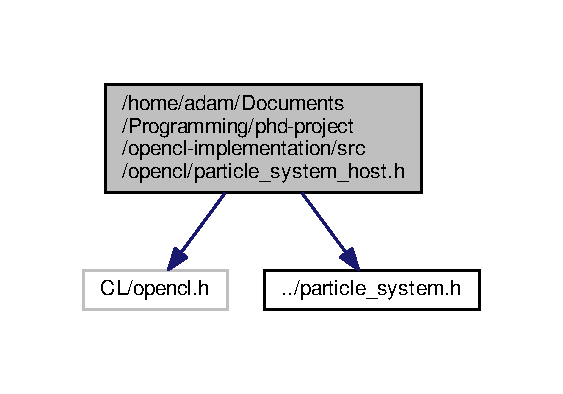
\includegraphics[width=270pt]{particle__system__host_8h__incl}
\end{center}
\end{figure}
This graph shows which files directly or indirectly include this file\+:
\nopagebreak
\begin{figure}[H]
\begin{center}
\leavevmode
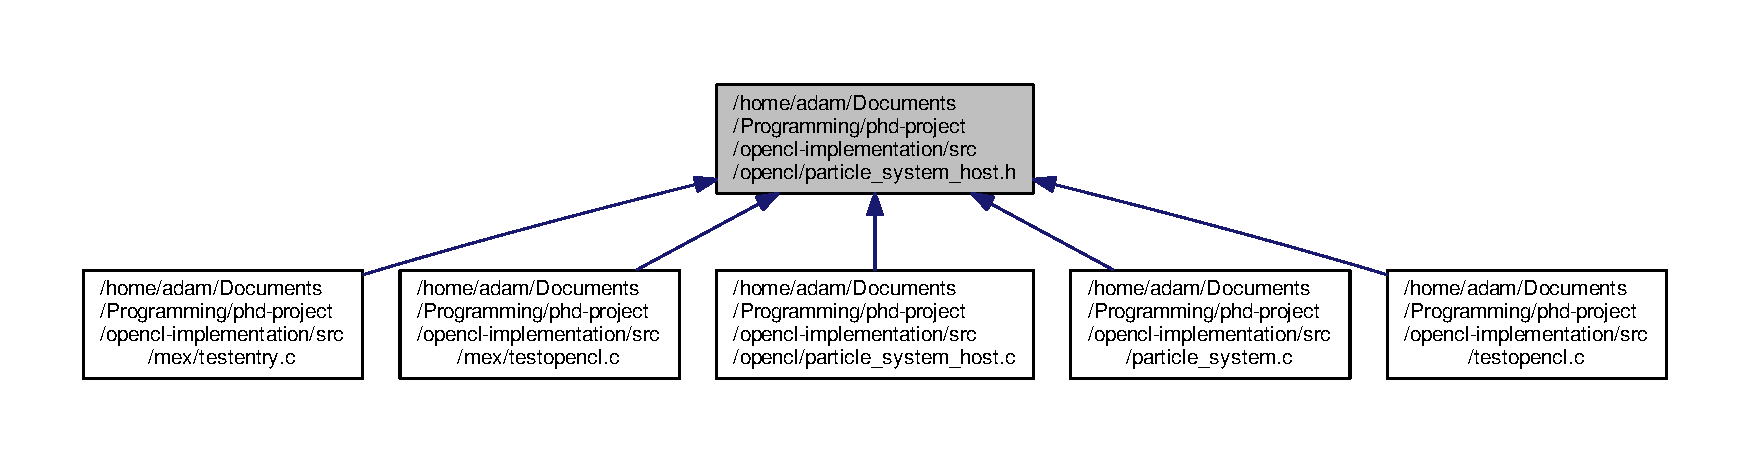
\includegraphics[width=350pt]{particle__system__host_8h__dep__incl}
\end{center}
\end{figure}
\subsection*{Data Structures}
\begin{DoxyCompactItemize}
\item 
struct \hyperlink{structpsdata__bufList}{psdata\+\_\+buf\+List}
\end{DoxyCompactItemize}
\subsection*{Functions}
\begin{DoxyCompactItemize}
\item 
void \hyperlink{particle__system__host_8h_a744914e82d7deaaab9366819f7570ace}{init\+\_\+ps\+\_\+opencl} ()
\item 
\hyperlink{structpsdata__bufList}{psdata\+\_\+buf\+List} \hyperlink{particle__system__host_8h_a0d894367a61fa9840cc6881b11578727}{create\+\_\+psdata\+\_\+opencl} ()
\item 
void \hyperlink{particle__system__host_8h_a264aaddb80e120e5ea4aee8685dc89ed}{opencl\+\_\+use\+\_\+buflist} (\hyperlink{structpsdata__bufList}{psdata\+\_\+buf\+List} bl)
\item 
void \hyperlink{particle__system__host_8h_a12619fd915a64b4a747df1a396a33449}{opencl\+\_\+set\+\_\+kernel\+\_\+buflist} (\hyperlink{structpsdata__bufList}{psdata\+\_\+buf\+List} bl, cl\+\_\+kernel kernel)
\item 
void \hyperlink{particle__system__host_8h_a7cedfb0b69b1ed8eea5ed8504385fdf8}{free\+\_\+psdata\+\_\+opencl} (\hyperlink{structpsdata__bufList}{psdata\+\_\+buf\+List} bl)
\item 
void \hyperlink{particle__system__host_8h_ae70d2a7474666f266b0ea73b278989bf}{terminate\+\_\+ps\+\_\+opencl} ()
\item 
void \hyperlink{particle__system__host_8h_a543f95a759ce9b341f399c0c7e52b909}{sync\+\_\+psdata\+\_\+device\+\_\+to\+\_\+host} (\hyperlink{structpsdata}{psdata} data, \hyperlink{structpsdata__bufList}{psdata\+\_\+buf\+List} bl)
\item 
void \hyperlink{particle__system__host_8h_a017aa0e283c0bb6ee128ff69cf10dd81}{sync\+\_\+psdata\+\_\+host\+\_\+to\+\_\+device} (\hyperlink{structpsdata}{psdata} data, \hyperlink{structpsdata__bufList}{psdata\+\_\+buf\+List} bl)
\item 
void \hyperlink{particle__system__host_8h_a2f9361e3844559923a7128b5c4770cc9}{populate\+\_\+position\+\_\+cuboid\+\_\+device\+\_\+opencl} (double x1, double y1, double z1, double x2, double y2, double z2, unsigned int xsize, unsigned int ysize, unsigned int zsize)
\item 
void \hyperlink{particle__system__host_8h_a2d2a85cfd370a03d94db3e13b6b1d2e0}{bin\+\_\+and\+\_\+sort\+\_\+device\+\_\+opencl} (\hyperlink{structpsdata}{psdata} $\ast$data)
\item 
void \hyperlink{particle__system__host_8h_a4dc67c508983e0050990d4d185f7791d}{bin\+\_\+particles\+\_\+device\+\_\+opencl} (\hyperlink{structpsdata}{psdata} $\ast$data)
\item 
void \hyperlink{particle__system__host_8h_a913da98edf2caadbdc7e74a2c04a72b9}{increment\+\_\+position\+\_\+0\+\_\+device\+\_\+opencl} ()
\item 
void \hyperlink{particle__system__host_8h_a385a5fd6747f1639c09f17df6791ebd5}{decrement\+\_\+position\+\_\+0\+\_\+device\+\_\+opencl} ()
\end{DoxyCompactItemize}


\subsection{Function Documentation}
\hypertarget{particle__system__host_8h_a2d2a85cfd370a03d94db3e13b6b1d2e0}{}\index{particle\+\_\+system\+\_\+host.\+h@{particle\+\_\+system\+\_\+host.\+h}!bin\+\_\+and\+\_\+sort\+\_\+device\+\_\+opencl@{bin\+\_\+and\+\_\+sort\+\_\+device\+\_\+opencl}}
\index{bin\+\_\+and\+\_\+sort\+\_\+device\+\_\+opencl@{bin\+\_\+and\+\_\+sort\+\_\+device\+\_\+opencl}!particle\+\_\+system\+\_\+host.\+h@{particle\+\_\+system\+\_\+host.\+h}}
\subsubsection[{bin\+\_\+and\+\_\+sort\+\_\+device\+\_\+opencl}]{\setlength{\rightskip}{0pt plus 5cm}void bin\+\_\+and\+\_\+sort\+\_\+device\+\_\+opencl (
\begin{DoxyParamCaption}
\item[{{\bf psdata} $\ast$}]{data}
\end{DoxyParamCaption}
)}\label{particle__system__host_8h_a2d2a85cfd370a03d94db3e13b6b1d2e0}
\hypertarget{particle__system__host_8h_a4dc67c508983e0050990d4d185f7791d}{}\index{particle\+\_\+system\+\_\+host.\+h@{particle\+\_\+system\+\_\+host.\+h}!bin\+\_\+particles\+\_\+device\+\_\+opencl@{bin\+\_\+particles\+\_\+device\+\_\+opencl}}
\index{bin\+\_\+particles\+\_\+device\+\_\+opencl@{bin\+\_\+particles\+\_\+device\+\_\+opencl}!particle\+\_\+system\+\_\+host.\+h@{particle\+\_\+system\+\_\+host.\+h}}
\subsubsection[{bin\+\_\+particles\+\_\+device\+\_\+opencl}]{\setlength{\rightskip}{0pt plus 5cm}void bin\+\_\+particles\+\_\+device\+\_\+opencl (
\begin{DoxyParamCaption}
\item[{{\bf psdata} $\ast$}]{data}
\end{DoxyParamCaption}
)}\label{particle__system__host_8h_a4dc67c508983e0050990d4d185f7791d}
\hypertarget{particle__system__host_8h_a0d894367a61fa9840cc6881b11578727}{}\index{particle\+\_\+system\+\_\+host.\+h@{particle\+\_\+system\+\_\+host.\+h}!create\+\_\+psdata\+\_\+opencl@{create\+\_\+psdata\+\_\+opencl}}
\index{create\+\_\+psdata\+\_\+opencl@{create\+\_\+psdata\+\_\+opencl}!particle\+\_\+system\+\_\+host.\+h@{particle\+\_\+system\+\_\+host.\+h}}
\subsubsection[{create\+\_\+psdata\+\_\+opencl}]{\setlength{\rightskip}{0pt plus 5cm}{\bf psdata\+\_\+buf\+List} create\+\_\+psdata\+\_\+opencl (
\begin{DoxyParamCaption}
{}
\end{DoxyParamCaption}
)}\label{particle__system__host_8h_a0d894367a61fa9840cc6881b11578727}
\hypertarget{particle__system__host_8h_a385a5fd6747f1639c09f17df6791ebd5}{}\index{particle\+\_\+system\+\_\+host.\+h@{particle\+\_\+system\+\_\+host.\+h}!decrement\+\_\+position\+\_\+0\+\_\+device\+\_\+opencl@{decrement\+\_\+position\+\_\+0\+\_\+device\+\_\+opencl}}
\index{decrement\+\_\+position\+\_\+0\+\_\+device\+\_\+opencl@{decrement\+\_\+position\+\_\+0\+\_\+device\+\_\+opencl}!particle\+\_\+system\+\_\+host.\+h@{particle\+\_\+system\+\_\+host.\+h}}
\subsubsection[{decrement\+\_\+position\+\_\+0\+\_\+device\+\_\+opencl}]{\setlength{\rightskip}{0pt plus 5cm}void decrement\+\_\+position\+\_\+0\+\_\+device\+\_\+opencl (
\begin{DoxyParamCaption}
{}
\end{DoxyParamCaption}
)}\label{particle__system__host_8h_a385a5fd6747f1639c09f17df6791ebd5}
\hypertarget{particle__system__host_8h_a7cedfb0b69b1ed8eea5ed8504385fdf8}{}\index{particle\+\_\+system\+\_\+host.\+h@{particle\+\_\+system\+\_\+host.\+h}!free\+\_\+psdata\+\_\+opencl@{free\+\_\+psdata\+\_\+opencl}}
\index{free\+\_\+psdata\+\_\+opencl@{free\+\_\+psdata\+\_\+opencl}!particle\+\_\+system\+\_\+host.\+h@{particle\+\_\+system\+\_\+host.\+h}}
\subsubsection[{free\+\_\+psdata\+\_\+opencl}]{\setlength{\rightskip}{0pt plus 5cm}void free\+\_\+psdata\+\_\+opencl (
\begin{DoxyParamCaption}
\item[{{\bf psdata\+\_\+buf\+List}}]{bl}
\end{DoxyParamCaption}
)}\label{particle__system__host_8h_a7cedfb0b69b1ed8eea5ed8504385fdf8}
Release referenced buffer \hypertarget{particle__system__host_8h_a913da98edf2caadbdc7e74a2c04a72b9}{}\index{particle\+\_\+system\+\_\+host.\+h@{particle\+\_\+system\+\_\+host.\+h}!increment\+\_\+position\+\_\+0\+\_\+device\+\_\+opencl@{increment\+\_\+position\+\_\+0\+\_\+device\+\_\+opencl}}
\index{increment\+\_\+position\+\_\+0\+\_\+device\+\_\+opencl@{increment\+\_\+position\+\_\+0\+\_\+device\+\_\+opencl}!particle\+\_\+system\+\_\+host.\+h@{particle\+\_\+system\+\_\+host.\+h}}
\subsubsection[{increment\+\_\+position\+\_\+0\+\_\+device\+\_\+opencl}]{\setlength{\rightskip}{0pt plus 5cm}void increment\+\_\+position\+\_\+0\+\_\+device\+\_\+opencl (
\begin{DoxyParamCaption}
{}
\end{DoxyParamCaption}
)}\label{particle__system__host_8h_a913da98edf2caadbdc7e74a2c04a72b9}
\hypertarget{particle__system__host_8h_a744914e82d7deaaab9366819f7570ace}{}\index{particle\+\_\+system\+\_\+host.\+h@{particle\+\_\+system\+\_\+host.\+h}!init\+\_\+ps\+\_\+opencl@{init\+\_\+ps\+\_\+opencl}}
\index{init\+\_\+ps\+\_\+opencl@{init\+\_\+ps\+\_\+opencl}!particle\+\_\+system\+\_\+host.\+h@{particle\+\_\+system\+\_\+host.\+h}}
\subsubsection[{init\+\_\+ps\+\_\+opencl}]{\setlength{\rightskip}{0pt plus 5cm}void init\+\_\+ps\+\_\+opencl (
\begin{DoxyParamCaption}
{}
\end{DoxyParamCaption}
)}\label{particle__system__host_8h_a744914e82d7deaaab9366819f7570ace}
Initialise Open\+C\+L

Detects hardware, creates command queues, compiles particle\+\_\+system\+\_\+kern.\+cl and creates kernels \hypertarget{particle__system__host_8h_a12619fd915a64b4a747df1a396a33449}{}\index{particle\+\_\+system\+\_\+host.\+h@{particle\+\_\+system\+\_\+host.\+h}!opencl\+\_\+set\+\_\+kernel\+\_\+buflist@{opencl\+\_\+set\+\_\+kernel\+\_\+buflist}}
\index{opencl\+\_\+set\+\_\+kernel\+\_\+buflist@{opencl\+\_\+set\+\_\+kernel\+\_\+buflist}!particle\+\_\+system\+\_\+host.\+h@{particle\+\_\+system\+\_\+host.\+h}}
\subsubsection[{opencl\+\_\+set\+\_\+kernel\+\_\+buflist}]{\setlength{\rightskip}{0pt plus 5cm}void opencl\+\_\+set\+\_\+kernel\+\_\+buflist (
\begin{DoxyParamCaption}
\item[{{\bf psdata\+\_\+buf\+List}}]{bl, }
\item[{cl\+\_\+kernel}]{kernel}
\end{DoxyParamCaption}
)}\label{particle__system__host_8h_a12619fd915a64b4a747df1a396a33449}
\hypertarget{particle__system__host_8h_a264aaddb80e120e5ea4aee8685dc89ed}{}\index{particle\+\_\+system\+\_\+host.\+h@{particle\+\_\+system\+\_\+host.\+h}!opencl\+\_\+use\+\_\+buflist@{opencl\+\_\+use\+\_\+buflist}}
\index{opencl\+\_\+use\+\_\+buflist@{opencl\+\_\+use\+\_\+buflist}!particle\+\_\+system\+\_\+host.\+h@{particle\+\_\+system\+\_\+host.\+h}}
\subsubsection[{opencl\+\_\+use\+\_\+buflist}]{\setlength{\rightskip}{0pt plus 5cm}void opencl\+\_\+use\+\_\+buflist (
\begin{DoxyParamCaption}
\item[{{\bf psdata\+\_\+buf\+List}}]{bl}
\end{DoxyParamCaption}
)}\label{particle__system__host_8h_a264aaddb80e120e5ea4aee8685dc89ed}
Use specified buffer in computations

Sets the arguments of kernels using psdata to this buflist


\begin{DoxyParams}{Parameters}
{\em bl} & Buffer list to use \\
\hline
\end{DoxyParams}
\hypertarget{particle__system__host_8h_a2f9361e3844559923a7128b5c4770cc9}{}\index{particle\+\_\+system\+\_\+host.\+h@{particle\+\_\+system\+\_\+host.\+h}!populate\+\_\+position\+\_\+cuboid\+\_\+device\+\_\+opencl@{populate\+\_\+position\+\_\+cuboid\+\_\+device\+\_\+opencl}}
\index{populate\+\_\+position\+\_\+cuboid\+\_\+device\+\_\+opencl@{populate\+\_\+position\+\_\+cuboid\+\_\+device\+\_\+opencl}!particle\+\_\+system\+\_\+host.\+h@{particle\+\_\+system\+\_\+host.\+h}}
\subsubsection[{populate\+\_\+position\+\_\+cuboid\+\_\+device\+\_\+opencl}]{\setlength{\rightskip}{0pt plus 5cm}void populate\+\_\+position\+\_\+cuboid\+\_\+device\+\_\+opencl (
\begin{DoxyParamCaption}
\item[{double}]{x1, }
\item[{double}]{y1, }
\item[{double}]{z1, }
\item[{double}]{x2, }
\item[{double}]{y2, }
\item[{double}]{z2, }
\item[{unsigned int}]{xsize, }
\item[{unsigned int}]{ysize, }
\item[{unsigned int}]{zsize}
\end{DoxyParamCaption}
)}\label{particle__system__host_8h_a2f9361e3844559923a7128b5c4770cc9}
\hypertarget{particle__system__host_8h_a543f95a759ce9b341f399c0c7e52b909}{}\index{particle\+\_\+system\+\_\+host.\+h@{particle\+\_\+system\+\_\+host.\+h}!sync\+\_\+psdata\+\_\+device\+\_\+to\+\_\+host@{sync\+\_\+psdata\+\_\+device\+\_\+to\+\_\+host}}
\index{sync\+\_\+psdata\+\_\+device\+\_\+to\+\_\+host@{sync\+\_\+psdata\+\_\+device\+\_\+to\+\_\+host}!particle\+\_\+system\+\_\+host.\+h@{particle\+\_\+system\+\_\+host.\+h}}
\subsubsection[{sync\+\_\+psdata\+\_\+device\+\_\+to\+\_\+host}]{\setlength{\rightskip}{0pt plus 5cm}void sync\+\_\+psdata\+\_\+device\+\_\+to\+\_\+host (
\begin{DoxyParamCaption}
\item[{{\bf psdata}}]{data, }
\item[{{\bf psdata\+\_\+buf\+List}}]{bl}
\end{DoxyParamCaption}
)}\label{particle__system__host_8h_a543f95a759ce9b341f399c0c7e52b909}
Copy buffer data from host to device


\begin{DoxyParams}{Parameters}
{\em data} & Host buffer \\
\hline
{\em bl} & \hyperlink{structDevice}{Device} buffer list \\
\hline
\end{DoxyParams}
\hypertarget{particle__system__host_8h_a017aa0e283c0bb6ee128ff69cf10dd81}{}\index{particle\+\_\+system\+\_\+host.\+h@{particle\+\_\+system\+\_\+host.\+h}!sync\+\_\+psdata\+\_\+host\+\_\+to\+\_\+device@{sync\+\_\+psdata\+\_\+host\+\_\+to\+\_\+device}}
\index{sync\+\_\+psdata\+\_\+host\+\_\+to\+\_\+device@{sync\+\_\+psdata\+\_\+host\+\_\+to\+\_\+device}!particle\+\_\+system\+\_\+host.\+h@{particle\+\_\+system\+\_\+host.\+h}}
\subsubsection[{sync\+\_\+psdata\+\_\+host\+\_\+to\+\_\+device}]{\setlength{\rightskip}{0pt plus 5cm}void sync\+\_\+psdata\+\_\+host\+\_\+to\+\_\+device (
\begin{DoxyParamCaption}
\item[{{\bf psdata}}]{data, }
\item[{{\bf psdata\+\_\+buf\+List}}]{bl}
\end{DoxyParamCaption}
)}\label{particle__system__host_8h_a017aa0e283c0bb6ee128ff69cf10dd81}
Copy buffer data from device to host


\begin{DoxyParams}{Parameters}
{\em data} & Host buffer \\
\hline
{\em bl} & \hyperlink{structDevice}{Device} buffer list \\
\hline
\end{DoxyParams}
\hypertarget{particle__system__host_8h_ae70d2a7474666f266b0ea73b278989bf}{}\index{particle\+\_\+system\+\_\+host.\+h@{particle\+\_\+system\+\_\+host.\+h}!terminate\+\_\+ps\+\_\+opencl@{terminate\+\_\+ps\+\_\+opencl}}
\index{terminate\+\_\+ps\+\_\+opencl@{terminate\+\_\+ps\+\_\+opencl}!particle\+\_\+system\+\_\+host.\+h@{particle\+\_\+system\+\_\+host.\+h}}
\subsubsection[{terminate\+\_\+ps\+\_\+opencl}]{\setlength{\rightskip}{0pt plus 5cm}void terminate\+\_\+ps\+\_\+opencl (
\begin{DoxyParamCaption}
{}
\end{DoxyParamCaption}
)}\label{particle__system__host_8h_ae70d2a7474666f266b0ea73b278989bf}
Terminate Open\+C\+L

Releases kernels, command queues and context. Does not release any buffers, though they may be invalid without the context. 
\hypertarget{platforminfo_8c}{}\section{/home/adam/\+Documents/\+Programming/phd-\/project/opencl-\/implementation/src/opencl/platforminfo.c File Reference}
\label{platforminfo_8c}\index{/home/adam/\+Documents/\+Programming/phd-\/project/opencl-\/implementation/src/opencl/platforminfo.\+c@{/home/adam/\+Documents/\+Programming/phd-\/project/opencl-\/implementation/src/opencl/platforminfo.\+c}}
{\ttfamily \#include $<$stdio.\+h$>$}\\*
{\ttfamily \#include $<$stdlib.\+h$>$}\\*
{\ttfamily \#include $<$string.\+h$>$}\\*
{\ttfamily \#include $<$C\+L/opencl.\+h$>$}\\*
{\ttfamily \#include \char`\"{}platforminfo.\+h\char`\"{}}\\*
{\ttfamily \#include \char`\"{}../note.\+h\char`\"{}}\\*
Include dependency graph for platforminfo.\+c\+:
\nopagebreak
\begin{figure}[H]
\begin{center}
\leavevmode
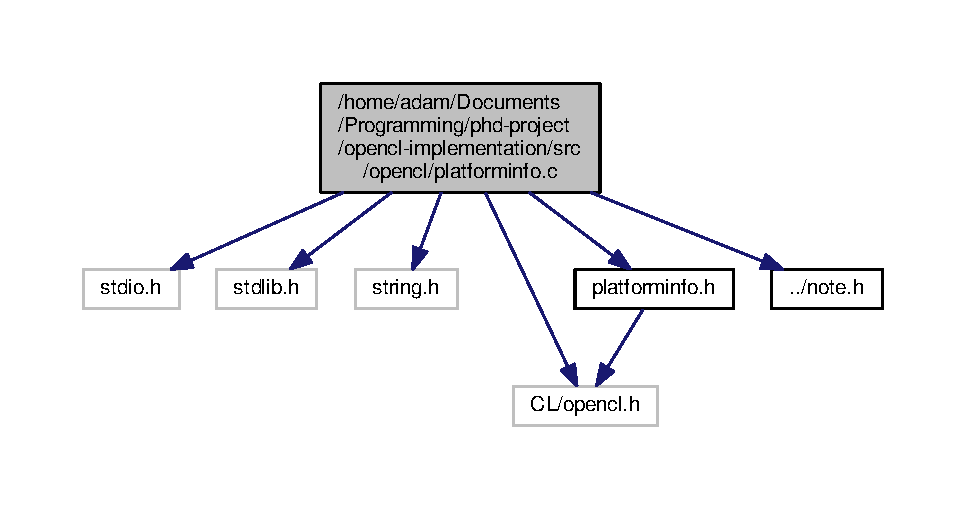
\includegraphics[width=350pt]{platforminfo_8c__incl}
\end{center}
\end{figure}
\subsection*{Functions}
\begin{DoxyCompactItemize}
\item 
void \hyperlink{platforminfo_8c_aaeaa39e62fd89a558420477f637a54c9}{get\+\_\+opencl\+\_\+platform\+\_\+info} (\hyperlink{structPlatform}{Platform} const $\ast$$\ast$const pptr, unsigned int $\ast$npptr)
\item 
void \hyperlink{platforminfo_8c_a30d1ad69c52bb0114f55438cdc2adbc9}{free\+\_\+opencl\+\_\+platform\+\_\+info} ()
\item 
char $\ast$ \hyperlink{platforminfo_8c_a7153ba5ecf1391a4d7fd509b290494d4}{get\+Device\+Info\+String} (cl\+\_\+device\+\_\+id, cl\+\_\+device\+\_\+info)
\item 
void \hyperlink{platforminfo_8c_a03f0381b3d478b0bdfa4329d826864f7}{print\+Device\+Type} (cl\+\_\+device\+\_\+type)
\item 
void \hyperlink{platforminfo_8c_acfbb69781e3884a68ac6dc509e7cc1f0}{print\+Device\+Bool} (cl\+\_\+bool)
\end{DoxyCompactItemize}


\subsection{Function Documentation}
\hypertarget{platforminfo_8c_a30d1ad69c52bb0114f55438cdc2adbc9}{}\index{platforminfo.\+c@{platforminfo.\+c}!free\+\_\+opencl\+\_\+platform\+\_\+info@{free\+\_\+opencl\+\_\+platform\+\_\+info}}
\index{free\+\_\+opencl\+\_\+platform\+\_\+info@{free\+\_\+opencl\+\_\+platform\+\_\+info}!platforminfo.\+c@{platforminfo.\+c}}
\subsubsection[{free\+\_\+opencl\+\_\+platform\+\_\+info}]{\setlength{\rightskip}{0pt plus 5cm}void free\+\_\+opencl\+\_\+platform\+\_\+info (
\begin{DoxyParamCaption}
{}
\end{DoxyParamCaption}
)}\label{platforminfo_8c_a30d1ad69c52bb0114f55438cdc2adbc9}
\hypertarget{platforminfo_8c_aaeaa39e62fd89a558420477f637a54c9}{}\index{platforminfo.\+c@{platforminfo.\+c}!get\+\_\+opencl\+\_\+platform\+\_\+info@{get\+\_\+opencl\+\_\+platform\+\_\+info}}
\index{get\+\_\+opencl\+\_\+platform\+\_\+info@{get\+\_\+opencl\+\_\+platform\+\_\+info}!platforminfo.\+c@{platforminfo.\+c}}
\subsubsection[{get\+\_\+opencl\+\_\+platform\+\_\+info}]{\setlength{\rightskip}{0pt plus 5cm}void get\+\_\+opencl\+\_\+platform\+\_\+info (
\begin{DoxyParamCaption}
\item[{{\bf Platform} const $\ast$$\ast$const}]{pptr, }
\item[{unsigned int $\ast$}]{npptr}
\end{DoxyParamCaption}
)}\label{platforminfo_8c_aaeaa39e62fd89a558420477f637a54c9}
\hypertarget{platforminfo_8c_a7153ba5ecf1391a4d7fd509b290494d4}{}\index{platforminfo.\+c@{platforminfo.\+c}!get\+Device\+Info\+String@{get\+Device\+Info\+String}}
\index{get\+Device\+Info\+String@{get\+Device\+Info\+String}!platforminfo.\+c@{platforminfo.\+c}}
\subsubsection[{get\+Device\+Info\+String}]{\setlength{\rightskip}{0pt plus 5cm}char $\ast$ get\+Device\+Info\+String (
\begin{DoxyParamCaption}
\item[{cl\+\_\+device\+\_\+id}]{device, }
\item[{cl\+\_\+device\+\_\+info}]{param\+\_\+name}
\end{DoxyParamCaption}
)}\label{platforminfo_8c_a7153ba5ecf1391a4d7fd509b290494d4}
\hypertarget{platforminfo_8c_acfbb69781e3884a68ac6dc509e7cc1f0}{}\index{platforminfo.\+c@{platforminfo.\+c}!print\+Device\+Bool@{print\+Device\+Bool}}
\index{print\+Device\+Bool@{print\+Device\+Bool}!platforminfo.\+c@{platforminfo.\+c}}
\subsubsection[{print\+Device\+Bool}]{\setlength{\rightskip}{0pt plus 5cm}void print\+Device\+Bool (
\begin{DoxyParamCaption}
\item[{cl\+\_\+bool}]{b}
\end{DoxyParamCaption}
)}\label{platforminfo_8c_acfbb69781e3884a68ac6dc509e7cc1f0}
\hypertarget{platforminfo_8c_a03f0381b3d478b0bdfa4329d826864f7}{}\index{platforminfo.\+c@{platforminfo.\+c}!print\+Device\+Type@{print\+Device\+Type}}
\index{print\+Device\+Type@{print\+Device\+Type}!platforminfo.\+c@{platforminfo.\+c}}
\subsubsection[{print\+Device\+Type}]{\setlength{\rightskip}{0pt plus 5cm}void print\+Device\+Type (
\begin{DoxyParamCaption}
\item[{cl\+\_\+device\+\_\+type}]{type}
\end{DoxyParamCaption}
)}\label{platforminfo_8c_a03f0381b3d478b0bdfa4329d826864f7}

\hypertarget{platforminfo_8h}{}\section{/home/adam/\+Documents/\+Programming/phd-\/project/opencl-\/implementation/src/opencl/platforminfo.h File Reference}
\label{platforminfo_8h}\index{/home/adam/\+Documents/\+Programming/phd-\/project/opencl-\/implementation/src/opencl/platforminfo.\+h@{/home/adam/\+Documents/\+Programming/phd-\/project/opencl-\/implementation/src/opencl/platforminfo.\+h}}
{\ttfamily \#include $<$C\+L/opencl.\+h$>$}\\*
Include dependency graph for platforminfo.\+h\+:
\nopagebreak
\begin{figure}[H]
\begin{center}
\leavevmode
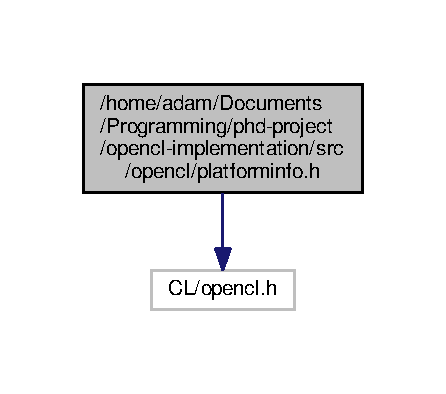
\includegraphics[width=214pt]{platforminfo_8h__incl}
\end{center}
\end{figure}
This graph shows which files directly or indirectly include this file\+:
\nopagebreak
\begin{figure}[H]
\begin{center}
\leavevmode
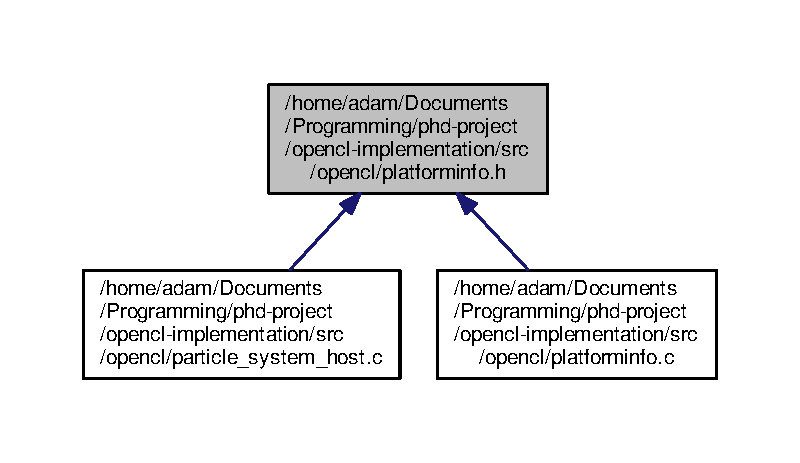
\includegraphics[width=350pt]{platforminfo_8h__dep__incl}
\end{center}
\end{figure}
\subsection*{Data Structures}
\begin{DoxyCompactItemize}
\item 
struct \hyperlink{structDevice}{Device}
\item 
struct \hyperlink{structPlatform}{Platform}
\end{DoxyCompactItemize}
\subsection*{Functions}
\begin{DoxyCompactItemize}
\item 
void \hyperlink{platforminfo_8h_a8e3d6d8dbc1963725f9bf35d15559706}{get\+\_\+opencl\+\_\+platform\+\_\+info} (\hyperlink{structPlatform}{Platform} const $\ast$$\ast$const pptr, unsigned int $\ast$const npptr)
\item 
void \hyperlink{platforminfo_8h_a30d1ad69c52bb0114f55438cdc2adbc9}{free\+\_\+opencl\+\_\+platform\+\_\+info} ()
\end{DoxyCompactItemize}


\subsection{Function Documentation}
\hypertarget{platforminfo_8h_a30d1ad69c52bb0114f55438cdc2adbc9}{}\index{platforminfo.\+h@{platforminfo.\+h}!free\+\_\+opencl\+\_\+platform\+\_\+info@{free\+\_\+opencl\+\_\+platform\+\_\+info}}
\index{free\+\_\+opencl\+\_\+platform\+\_\+info@{free\+\_\+opencl\+\_\+platform\+\_\+info}!platforminfo.\+h@{platforminfo.\+h}}
\subsubsection[{free\+\_\+opencl\+\_\+platform\+\_\+info}]{\setlength{\rightskip}{0pt plus 5cm}void free\+\_\+opencl\+\_\+platform\+\_\+info (
\begin{DoxyParamCaption}
{}
\end{DoxyParamCaption}
)}\label{platforminfo_8h_a30d1ad69c52bb0114f55438cdc2adbc9}
\hypertarget{platforminfo_8h_a8e3d6d8dbc1963725f9bf35d15559706}{}\index{platforminfo.\+h@{platforminfo.\+h}!get\+\_\+opencl\+\_\+platform\+\_\+info@{get\+\_\+opencl\+\_\+platform\+\_\+info}}
\index{get\+\_\+opencl\+\_\+platform\+\_\+info@{get\+\_\+opencl\+\_\+platform\+\_\+info}!platforminfo.\+h@{platforminfo.\+h}}
\subsubsection[{get\+\_\+opencl\+\_\+platform\+\_\+info}]{\setlength{\rightskip}{0pt plus 5cm}void get\+\_\+opencl\+\_\+platform\+\_\+info (
\begin{DoxyParamCaption}
\item[{{\bf Platform} const $\ast$$\ast$const}]{pptr, }
\item[{unsigned int $\ast$const}]{npptr}
\end{DoxyParamCaption}
)}\label{platforminfo_8h_a8e3d6d8dbc1963725f9bf35d15559706}

\hypertarget{particle__system_8c}{}\section{/home/adam/\+Documents/\+Programming/phd-\/project/opencl-\/implementation/src/particle\+\_\+system.c File Reference}
\label{particle__system_8c}\index{/home/adam/\+Documents/\+Programming/phd-\/project/opencl-\/implementation/src/particle\+\_\+system.\+c@{/home/adam/\+Documents/\+Programming/phd-\/project/opencl-\/implementation/src/particle\+\_\+system.\+c}}
{\ttfamily \#include $<$math.\+h$>$}\\*
{\ttfamily \#include $<$string.\+h$>$}\\*
{\ttfamily \#include $<$stdlib.\+h$>$}\\*
{\ttfamily \#include \char`\"{}particle\+\_\+system.\+h\char`\"{}}\\*
{\ttfamily \#include \char`\"{}opencl/particle\+\_\+system\+\_\+host.\+h\char`\"{}}\\*
Include dependency graph for particle\+\_\+system.\+c\+:
\nopagebreak
\begin{figure}[H]
\begin{center}
\leavevmode
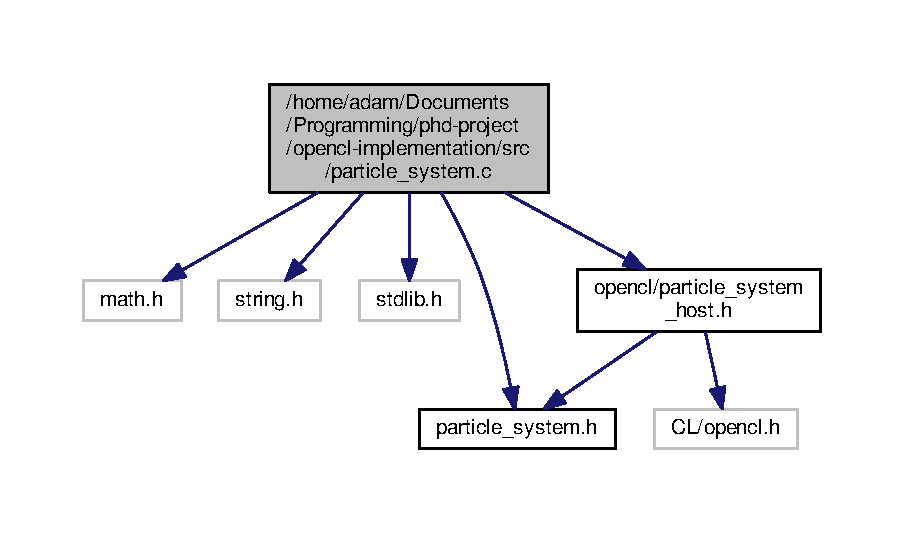
\includegraphics[width=350pt]{particle__system_8c__incl}
\end{center}
\end{figure}
\subsection*{Functions}
\begin{DoxyCompactItemize}
\item 
void \hyperlink{particle__system_8c_aeea6607d3297e41f5eb21f0401fd8abe}{init\+\_\+psdata\+\_\+fluid} (\hyperlink{structpsdata}{psdata} $\ast$data, int pnum, double mass, double timestep, double smoothingradius, double xbound1, double ybound1, double zbound1, double xbound2, double ybound2, double zbound2)
\item 
int \hyperlink{particle__system_8c_a93f226a57d8b95e4ecac03eace11362c}{get\+\_\+field\+\_\+psdata} (\hyperlink{structpsdata}{psdata} $\ast$data, const char $\ast$name)
\item 
void \hyperlink{particle__system_8c_abe0f70f47b2ffc0df6cb70dd6333bd1e}{set\+\_\+field\+\_\+psdata} (\hyperlink{structpsdata}{psdata} $\ast$data, const char $\ast$name, void $\ast$field, unsigned int size, unsigned int offset)
\item 
unsigned int \hyperlink{particle__system_8c_ae8b07c803b148cd6e82a0d5a00dde9e2}{psdata\+\_\+names\+\_\+size} (\hyperlink{structpsdata}{psdata} $\ast$data)
\item 
unsigned int \hyperlink{particle__system_8c_ae7da24b83abcc08aec97401d6f7f1578}{psdata\+\_\+dimensions\+\_\+size} (\hyperlink{structpsdata}{psdata} $\ast$data)
\item 
unsigned int \hyperlink{particle__system_8c_af64d7fa0124689bb86acb3da1f662e7c}{psdata\+\_\+data\+\_\+size} (\hyperlink{structpsdata}{psdata} $\ast$data)
\item 
int \hyperlink{particle__system_8c_a126f49b5c03518c67612e297508b37d3}{create\+\_\+host\+\_\+field\+\_\+psdata} (\hyperlink{structpsdata}{psdata} $\ast$data, const char $\ast$name, void $\ast$field, unsigned int size)
\item 
int \hyperlink{particle__system_8c_a4f82b0221d392d80cbf64f4389989c84}{get\+\_\+host\+\_\+field\+\_\+psdata} (\hyperlink{structpsdata}{psdata} $\ast$data, const char $\ast$name)
\item 
void \hyperlink{particle__system_8c_ac9bf17eff0cc5aa4ff695b89c19043c3}{free\+\_\+psdata} (\hyperlink{structpsdata}{psdata} data)
\end{DoxyCompactItemize}


\subsection{Function Documentation}
\hypertarget{particle__system_8c_a126f49b5c03518c67612e297508b37d3}{}\index{particle\+\_\+system.\+c@{particle\+\_\+system.\+c}!create\+\_\+host\+\_\+field\+\_\+psdata@{create\+\_\+host\+\_\+field\+\_\+psdata}}
\index{create\+\_\+host\+\_\+field\+\_\+psdata@{create\+\_\+host\+\_\+field\+\_\+psdata}!particle\+\_\+system.\+c@{particle\+\_\+system.\+c}}
\subsubsection[{create\+\_\+host\+\_\+field\+\_\+psdata}]{\setlength{\rightskip}{0pt plus 5cm}int create\+\_\+host\+\_\+field\+\_\+psdata (
\begin{DoxyParamCaption}
\item[{{\bf psdata} $\ast$}]{data, }
\item[{const char $\ast$}]{name, }
\item[{void $\ast$}]{field, }
\item[{unsigned int}]{size}
\end{DoxyParamCaption}
)}\label{particle__system_8c_a126f49b5c03518c67612e297508b37d3}
\hypertarget{particle__system_8c_ac9bf17eff0cc5aa4ff695b89c19043c3}{}\index{particle\+\_\+system.\+c@{particle\+\_\+system.\+c}!free\+\_\+psdata@{free\+\_\+psdata}}
\index{free\+\_\+psdata@{free\+\_\+psdata}!particle\+\_\+system.\+c@{particle\+\_\+system.\+c}}
\subsubsection[{free\+\_\+psdata}]{\setlength{\rightskip}{0pt plus 5cm}void free\+\_\+psdata (
\begin{DoxyParamCaption}
\item[{{\bf psdata}}]{data}
\end{DoxyParamCaption}
)}\label{particle__system_8c_ac9bf17eff0cc5aa4ff695b89c19043c3}
\hypertarget{particle__system_8c_a93f226a57d8b95e4ecac03eace11362c}{}\index{particle\+\_\+system.\+c@{particle\+\_\+system.\+c}!get\+\_\+field\+\_\+psdata@{get\+\_\+field\+\_\+psdata}}
\index{get\+\_\+field\+\_\+psdata@{get\+\_\+field\+\_\+psdata}!particle\+\_\+system.\+c@{particle\+\_\+system.\+c}}
\subsubsection[{get\+\_\+field\+\_\+psdata}]{\setlength{\rightskip}{0pt plus 5cm}int get\+\_\+field\+\_\+psdata (
\begin{DoxyParamCaption}
\item[{{\bf psdata} $\ast$}]{data, }
\item[{const char $\ast$}]{name}
\end{DoxyParamCaption}
)}\label{particle__system_8c_a93f226a57d8b95e4ecac03eace11362c}
\hypertarget{particle__system_8c_a4f82b0221d392d80cbf64f4389989c84}{}\index{particle\+\_\+system.\+c@{particle\+\_\+system.\+c}!get\+\_\+host\+\_\+field\+\_\+psdata@{get\+\_\+host\+\_\+field\+\_\+psdata}}
\index{get\+\_\+host\+\_\+field\+\_\+psdata@{get\+\_\+host\+\_\+field\+\_\+psdata}!particle\+\_\+system.\+c@{particle\+\_\+system.\+c}}
\subsubsection[{get\+\_\+host\+\_\+field\+\_\+psdata}]{\setlength{\rightskip}{0pt plus 5cm}int get\+\_\+host\+\_\+field\+\_\+psdata (
\begin{DoxyParamCaption}
\item[{{\bf psdata} $\ast$}]{data, }
\item[{const char $\ast$}]{name}
\end{DoxyParamCaption}
)}\label{particle__system_8c_a4f82b0221d392d80cbf64f4389989c84}
\hypertarget{particle__system_8c_aeea6607d3297e41f5eb21f0401fd8abe}{}\index{particle\+\_\+system.\+c@{particle\+\_\+system.\+c}!init\+\_\+psdata\+\_\+fluid@{init\+\_\+psdata\+\_\+fluid}}
\index{init\+\_\+psdata\+\_\+fluid@{init\+\_\+psdata\+\_\+fluid}!particle\+\_\+system.\+c@{particle\+\_\+system.\+c}}
\subsubsection[{init\+\_\+psdata\+\_\+fluid}]{\setlength{\rightskip}{0pt plus 5cm}void init\+\_\+psdata\+\_\+fluid (
\begin{DoxyParamCaption}
\item[{{\bf psdata} $\ast$}]{data, }
\item[{int}]{pnum, }
\item[{double}]{mass, }
\item[{double}]{timestep, }
\item[{double}]{smoothingradius, }
\item[{double}]{xbound1, }
\item[{double}]{ybound1, }
\item[{double}]{zbound1, }
\item[{double}]{xbound2, }
\item[{double}]{ybound2, }
\item[{double}]{zbound2}
\end{DoxyParamCaption}
)}\label{particle__system_8c_aeea6607d3297e41f5eb21f0401fd8abe}
\hypertarget{particle__system_8c_af64d7fa0124689bb86acb3da1f662e7c}{}\index{particle\+\_\+system.\+c@{particle\+\_\+system.\+c}!psdata\+\_\+data\+\_\+size@{psdata\+\_\+data\+\_\+size}}
\index{psdata\+\_\+data\+\_\+size@{psdata\+\_\+data\+\_\+size}!particle\+\_\+system.\+c@{particle\+\_\+system.\+c}}
\subsubsection[{psdata\+\_\+data\+\_\+size}]{\setlength{\rightskip}{0pt plus 5cm}unsigned int psdata\+\_\+data\+\_\+size (
\begin{DoxyParamCaption}
\item[{{\bf psdata} $\ast$}]{data}
\end{DoxyParamCaption}
)}\label{particle__system_8c_af64d7fa0124689bb86acb3da1f662e7c}
\hypertarget{particle__system_8c_ae7da24b83abcc08aec97401d6f7f1578}{}\index{particle\+\_\+system.\+c@{particle\+\_\+system.\+c}!psdata\+\_\+dimensions\+\_\+size@{psdata\+\_\+dimensions\+\_\+size}}
\index{psdata\+\_\+dimensions\+\_\+size@{psdata\+\_\+dimensions\+\_\+size}!particle\+\_\+system.\+c@{particle\+\_\+system.\+c}}
\subsubsection[{psdata\+\_\+dimensions\+\_\+size}]{\setlength{\rightskip}{0pt plus 5cm}unsigned int psdata\+\_\+dimensions\+\_\+size (
\begin{DoxyParamCaption}
\item[{{\bf psdata} $\ast$}]{data}
\end{DoxyParamCaption}
)}\label{particle__system_8c_ae7da24b83abcc08aec97401d6f7f1578}
\hypertarget{particle__system_8c_ae8b07c803b148cd6e82a0d5a00dde9e2}{}\index{particle\+\_\+system.\+c@{particle\+\_\+system.\+c}!psdata\+\_\+names\+\_\+size@{psdata\+\_\+names\+\_\+size}}
\index{psdata\+\_\+names\+\_\+size@{psdata\+\_\+names\+\_\+size}!particle\+\_\+system.\+c@{particle\+\_\+system.\+c}}
\subsubsection[{psdata\+\_\+names\+\_\+size}]{\setlength{\rightskip}{0pt plus 5cm}unsigned int psdata\+\_\+names\+\_\+size (
\begin{DoxyParamCaption}
\item[{{\bf psdata} $\ast$}]{data}
\end{DoxyParamCaption}
)}\label{particle__system_8c_ae8b07c803b148cd6e82a0d5a00dde9e2}
\hypertarget{particle__system_8c_abe0f70f47b2ffc0df6cb70dd6333bd1e}{}\index{particle\+\_\+system.\+c@{particle\+\_\+system.\+c}!set\+\_\+field\+\_\+psdata@{set\+\_\+field\+\_\+psdata}}
\index{set\+\_\+field\+\_\+psdata@{set\+\_\+field\+\_\+psdata}!particle\+\_\+system.\+c@{particle\+\_\+system.\+c}}
\subsubsection[{set\+\_\+field\+\_\+psdata}]{\setlength{\rightskip}{0pt plus 5cm}void set\+\_\+field\+\_\+psdata (
\begin{DoxyParamCaption}
\item[{{\bf psdata} $\ast$}]{data, }
\item[{const char $\ast$}]{name, }
\item[{void $\ast$}]{field, }
\item[{unsigned int}]{size, }
\item[{unsigned int}]{offset}
\end{DoxyParamCaption}
)}\label{particle__system_8c_abe0f70f47b2ffc0df6cb70dd6333bd1e}

\hypertarget{particle__system_8h}{}\section{/home/adam/\+Documents/\+Programming/phd-\/project/opencl-\/implementation/src/particle\+\_\+system.h File Reference}
\label{particle__system_8h}\index{/home/adam/\+Documents/\+Programming/phd-\/project/opencl-\/implementation/src/particle\+\_\+system.\+h@{/home/adam/\+Documents/\+Programming/phd-\/project/opencl-\/implementation/src/particle\+\_\+system.\+h}}
This graph shows which files directly or indirectly include this file\+:
\nopagebreak
\begin{figure}[H]
\begin{center}
\leavevmode
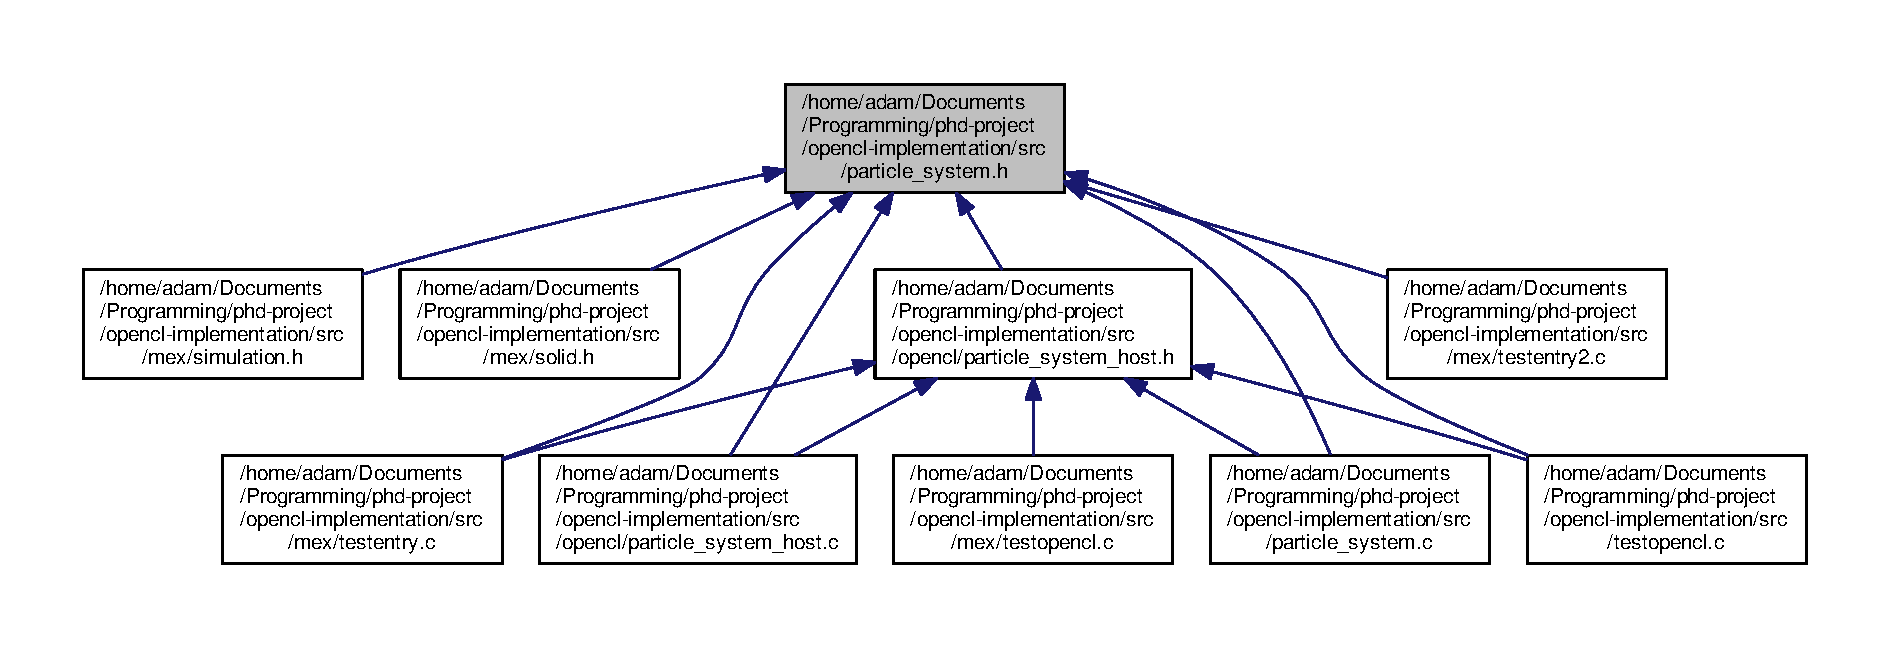
\includegraphics[width=350pt]{particle__system_8h__dep__incl}
\end{center}
\end{figure}
\subsection*{Data Structures}
\begin{DoxyCompactItemize}
\item 
struct \hyperlink{structpsdata}{psdata}
\end{DoxyCompactItemize}
\subsection*{Macros}
\begin{DoxyCompactItemize}
\item 
\#define \hyperlink{particle__system_8h_ac3fcd481ecbc5730f9385f2526c58718}{P\+S\+\_\+\+P\+\_\+\+P\+T\+R}(d,  position,  type)~((type$\ast$) ((char$\ast$) d-\/$>$data + d-\/$>$data\+\_\+offsets\mbox{[}position\mbox{]}))
\item 
\#define \hyperlink{particle__system_8h_a8fa6065663aa7ea3abf11eb542cbd02f}{P\+S\+\_\+\+S\+E\+T\+\_\+\+P\+T\+R}(data,  name,  type,  pointer\+\_\+to\+\_\+pointer)
\end{DoxyCompactItemize}
\subsection*{Functions}
\begin{DoxyCompactItemize}
\item 
void \hyperlink{particle__system_8h_aeea6607d3297e41f5eb21f0401fd8abe}{init\+\_\+psdata\+\_\+fluid} (\hyperlink{structpsdata}{psdata} $\ast$data, int pnum, double mass, double timestep, double smoothingradius, double xbound1, double ybound1, double zbound1, double xbound2, double ybound2, double zbound2)
\item 
int \hyperlink{particle__system_8h_a93f226a57d8b95e4ecac03eace11362c}{get\+\_\+field\+\_\+psdata} (\hyperlink{structpsdata}{psdata} $\ast$data, const char $\ast$name)
\item 
void \hyperlink{particle__system_8h_abe0f70f47b2ffc0df6cb70dd6333bd1e}{set\+\_\+field\+\_\+psdata} (\hyperlink{structpsdata}{psdata} $\ast$data, const char $\ast$name, void $\ast$field, unsigned int size, unsigned int offset)
\item 
unsigned int \hyperlink{particle__system_8h_ae8b07c803b148cd6e82a0d5a00dde9e2}{psdata\+\_\+names\+\_\+size} (\hyperlink{structpsdata}{psdata} $\ast$data)
\item 
unsigned int \hyperlink{particle__system_8h_ae7da24b83abcc08aec97401d6f7f1578}{psdata\+\_\+dimensions\+\_\+size} (\hyperlink{structpsdata}{psdata} $\ast$data)
\item 
unsigned int \hyperlink{particle__system_8h_af64d7fa0124689bb86acb3da1f662e7c}{psdata\+\_\+data\+\_\+size} (\hyperlink{structpsdata}{psdata} $\ast$data)
\item 
int \hyperlink{particle__system_8h_a126f49b5c03518c67612e297508b37d3}{create\+\_\+host\+\_\+field\+\_\+psdata} (\hyperlink{structpsdata}{psdata} $\ast$data, const char $\ast$name, void $\ast$field, unsigned int size)
\item 
int \hyperlink{particle__system_8h_a4f82b0221d392d80cbf64f4389989c84}{get\+\_\+host\+\_\+field\+\_\+psdata} (\hyperlink{structpsdata}{psdata} $\ast$data, const char $\ast$name)
\item 
void \hyperlink{particle__system_8h_ac9bf17eff0cc5aa4ff695b89c19043c3}{free\+\_\+psdata} (\hyperlink{structpsdata}{psdata} data)
\end{DoxyCompactItemize}


\subsection{Macro Definition Documentation}
\hypertarget{particle__system_8h_ac3fcd481ecbc5730f9385f2526c58718}{}\index{particle\+\_\+system.\+h@{particle\+\_\+system.\+h}!P\+S\+\_\+\+P\+\_\+\+P\+T\+R@{P\+S\+\_\+\+P\+\_\+\+P\+T\+R}}
\index{P\+S\+\_\+\+P\+\_\+\+P\+T\+R@{P\+S\+\_\+\+P\+\_\+\+P\+T\+R}!particle\+\_\+system.\+h@{particle\+\_\+system.\+h}}
\subsubsection[{P\+S\+\_\+\+P\+\_\+\+P\+T\+R}]{\setlength{\rightskip}{0pt plus 5cm}\#define P\+S\+\_\+\+P\+\_\+\+P\+T\+R(
\begin{DoxyParamCaption}
\item[{}]{d, }
\item[{}]{position, }
\item[{}]{type}
\end{DoxyParamCaption}
)~((type$\ast$) ((char$\ast$) d-\/$>$data + d-\/$>$data\+\_\+offsets\mbox{[}position\mbox{]}))}\label{particle__system_8h_ac3fcd481ecbc5730f9385f2526c58718}
\hypertarget{particle__system_8h_a8fa6065663aa7ea3abf11eb542cbd02f}{}\index{particle\+\_\+system.\+h@{particle\+\_\+system.\+h}!P\+S\+\_\+\+S\+E\+T\+\_\+\+P\+T\+R@{P\+S\+\_\+\+S\+E\+T\+\_\+\+P\+T\+R}}
\index{P\+S\+\_\+\+S\+E\+T\+\_\+\+P\+T\+R@{P\+S\+\_\+\+S\+E\+T\+\_\+\+P\+T\+R}!particle\+\_\+system.\+h@{particle\+\_\+system.\+h}}
\subsubsection[{P\+S\+\_\+\+S\+E\+T\+\_\+\+P\+T\+R}]{\setlength{\rightskip}{0pt plus 5cm}\#define P\+S\+\_\+\+S\+E\+T\+\_\+\+P\+T\+R(
\begin{DoxyParamCaption}
\item[{}]{data, }
\item[{}]{name, }
\item[{}]{type, }
\item[{}]{pointer\+\_\+to\+\_\+pointer}
\end{DoxyParamCaption}
)}\label{particle__system_8h_a8fa6065663aa7ea3abf11eb542cbd02f}
{\bfseries Value\+:}
\begin{DoxyCode}
\{\(\backslash\)
    int \_\_fldpos = \hyperlink{particle__system_8h_a93f226a57d8b95e4ecac03eace11362c}{get\_field\_psdata}(data, name); \(\backslash\)
    assert(\_\_fldpos != -1); \(\backslash\)
    *pointer\_to\_pointer = \hyperlink{particle__system_8h_ac3fcd481ecbc5730f9385f2526c58718}{PS\_P\_PTR}(data, \_\_fldpos, type);\}
\end{DoxyCode}


\subsection{Function Documentation}
\hypertarget{particle__system_8h_a126f49b5c03518c67612e297508b37d3}{}\index{particle\+\_\+system.\+h@{particle\+\_\+system.\+h}!create\+\_\+host\+\_\+field\+\_\+psdata@{create\+\_\+host\+\_\+field\+\_\+psdata}}
\index{create\+\_\+host\+\_\+field\+\_\+psdata@{create\+\_\+host\+\_\+field\+\_\+psdata}!particle\+\_\+system.\+h@{particle\+\_\+system.\+h}}
\subsubsection[{create\+\_\+host\+\_\+field\+\_\+psdata}]{\setlength{\rightskip}{0pt plus 5cm}int create\+\_\+host\+\_\+field\+\_\+psdata (
\begin{DoxyParamCaption}
\item[{{\bf psdata} $\ast$}]{data, }
\item[{const char $\ast$}]{name, }
\item[{void $\ast$}]{field, }
\item[{unsigned int}]{size}
\end{DoxyParamCaption}
)}\label{particle__system_8h_a126f49b5c03518c67612e297508b37d3}
\hypertarget{particle__system_8h_ac9bf17eff0cc5aa4ff695b89c19043c3}{}\index{particle\+\_\+system.\+h@{particle\+\_\+system.\+h}!free\+\_\+psdata@{free\+\_\+psdata}}
\index{free\+\_\+psdata@{free\+\_\+psdata}!particle\+\_\+system.\+h@{particle\+\_\+system.\+h}}
\subsubsection[{free\+\_\+psdata}]{\setlength{\rightskip}{0pt plus 5cm}void free\+\_\+psdata (
\begin{DoxyParamCaption}
\item[{{\bf psdata}}]{data}
\end{DoxyParamCaption}
)}\label{particle__system_8h_ac9bf17eff0cc5aa4ff695b89c19043c3}
\hypertarget{particle__system_8h_a93f226a57d8b95e4ecac03eace11362c}{}\index{particle\+\_\+system.\+h@{particle\+\_\+system.\+h}!get\+\_\+field\+\_\+psdata@{get\+\_\+field\+\_\+psdata}}
\index{get\+\_\+field\+\_\+psdata@{get\+\_\+field\+\_\+psdata}!particle\+\_\+system.\+h@{particle\+\_\+system.\+h}}
\subsubsection[{get\+\_\+field\+\_\+psdata}]{\setlength{\rightskip}{0pt plus 5cm}int get\+\_\+field\+\_\+psdata (
\begin{DoxyParamCaption}
\item[{{\bf psdata} $\ast$}]{data, }
\item[{const char $\ast$}]{name}
\end{DoxyParamCaption}
)}\label{particle__system_8h_a93f226a57d8b95e4ecac03eace11362c}
\hypertarget{particle__system_8h_a4f82b0221d392d80cbf64f4389989c84}{}\index{particle\+\_\+system.\+h@{particle\+\_\+system.\+h}!get\+\_\+host\+\_\+field\+\_\+psdata@{get\+\_\+host\+\_\+field\+\_\+psdata}}
\index{get\+\_\+host\+\_\+field\+\_\+psdata@{get\+\_\+host\+\_\+field\+\_\+psdata}!particle\+\_\+system.\+h@{particle\+\_\+system.\+h}}
\subsubsection[{get\+\_\+host\+\_\+field\+\_\+psdata}]{\setlength{\rightskip}{0pt plus 5cm}int get\+\_\+host\+\_\+field\+\_\+psdata (
\begin{DoxyParamCaption}
\item[{{\bf psdata} $\ast$}]{data, }
\item[{const char $\ast$}]{name}
\end{DoxyParamCaption}
)}\label{particle__system_8h_a4f82b0221d392d80cbf64f4389989c84}
\hypertarget{particle__system_8h_aeea6607d3297e41f5eb21f0401fd8abe}{}\index{particle\+\_\+system.\+h@{particle\+\_\+system.\+h}!init\+\_\+psdata\+\_\+fluid@{init\+\_\+psdata\+\_\+fluid}}
\index{init\+\_\+psdata\+\_\+fluid@{init\+\_\+psdata\+\_\+fluid}!particle\+\_\+system.\+h@{particle\+\_\+system.\+h}}
\subsubsection[{init\+\_\+psdata\+\_\+fluid}]{\setlength{\rightskip}{0pt plus 5cm}void init\+\_\+psdata\+\_\+fluid (
\begin{DoxyParamCaption}
\item[{{\bf psdata} $\ast$}]{data, }
\item[{int}]{pnum, }
\item[{double}]{mass, }
\item[{double}]{timestep, }
\item[{double}]{smoothingradius, }
\item[{double}]{xbound1, }
\item[{double}]{ybound1, }
\item[{double}]{zbound1, }
\item[{double}]{xbound2, }
\item[{double}]{ybound2, }
\item[{double}]{zbound2}
\end{DoxyParamCaption}
)}\label{particle__system_8h_aeea6607d3297e41f5eb21f0401fd8abe}
\hypertarget{particle__system_8h_af64d7fa0124689bb86acb3da1f662e7c}{}\index{particle\+\_\+system.\+h@{particle\+\_\+system.\+h}!psdata\+\_\+data\+\_\+size@{psdata\+\_\+data\+\_\+size}}
\index{psdata\+\_\+data\+\_\+size@{psdata\+\_\+data\+\_\+size}!particle\+\_\+system.\+h@{particle\+\_\+system.\+h}}
\subsubsection[{psdata\+\_\+data\+\_\+size}]{\setlength{\rightskip}{0pt plus 5cm}unsigned int psdata\+\_\+data\+\_\+size (
\begin{DoxyParamCaption}
\item[{{\bf psdata} $\ast$}]{data}
\end{DoxyParamCaption}
)}\label{particle__system_8h_af64d7fa0124689bb86acb3da1f662e7c}
\hypertarget{particle__system_8h_ae7da24b83abcc08aec97401d6f7f1578}{}\index{particle\+\_\+system.\+h@{particle\+\_\+system.\+h}!psdata\+\_\+dimensions\+\_\+size@{psdata\+\_\+dimensions\+\_\+size}}
\index{psdata\+\_\+dimensions\+\_\+size@{psdata\+\_\+dimensions\+\_\+size}!particle\+\_\+system.\+h@{particle\+\_\+system.\+h}}
\subsubsection[{psdata\+\_\+dimensions\+\_\+size}]{\setlength{\rightskip}{0pt plus 5cm}unsigned int psdata\+\_\+dimensions\+\_\+size (
\begin{DoxyParamCaption}
\item[{{\bf psdata} $\ast$}]{data}
\end{DoxyParamCaption}
)}\label{particle__system_8h_ae7da24b83abcc08aec97401d6f7f1578}
\hypertarget{particle__system_8h_ae8b07c803b148cd6e82a0d5a00dde9e2}{}\index{particle\+\_\+system.\+h@{particle\+\_\+system.\+h}!psdata\+\_\+names\+\_\+size@{psdata\+\_\+names\+\_\+size}}
\index{psdata\+\_\+names\+\_\+size@{psdata\+\_\+names\+\_\+size}!particle\+\_\+system.\+h@{particle\+\_\+system.\+h}}
\subsubsection[{psdata\+\_\+names\+\_\+size}]{\setlength{\rightskip}{0pt plus 5cm}unsigned int psdata\+\_\+names\+\_\+size (
\begin{DoxyParamCaption}
\item[{{\bf psdata} $\ast$}]{data}
\end{DoxyParamCaption}
)}\label{particle__system_8h_ae8b07c803b148cd6e82a0d5a00dde9e2}
\hypertarget{particle__system_8h_abe0f70f47b2ffc0df6cb70dd6333bd1e}{}\index{particle\+\_\+system.\+h@{particle\+\_\+system.\+h}!set\+\_\+field\+\_\+psdata@{set\+\_\+field\+\_\+psdata}}
\index{set\+\_\+field\+\_\+psdata@{set\+\_\+field\+\_\+psdata}!particle\+\_\+system.\+h@{particle\+\_\+system.\+h}}
\subsubsection[{set\+\_\+field\+\_\+psdata}]{\setlength{\rightskip}{0pt plus 5cm}void set\+\_\+field\+\_\+psdata (
\begin{DoxyParamCaption}
\item[{{\bf psdata} $\ast$}]{data, }
\item[{const char $\ast$}]{name, }
\item[{void $\ast$}]{field, }
\item[{unsigned int}]{size, }
\item[{unsigned int}]{offset}
\end{DoxyParamCaption}
)}\label{particle__system_8h_abe0f70f47b2ffc0df6cb70dd6333bd1e}

%--- End generated contents ---

% Index
\backmatter
\newpage
\phantomsection
\clearemptydoublepage
\addcontentsline{toc}{chapter}{Index}
\printindex

\end{document}
